% Options for packages loaded elsewhere
\PassOptionsToPackage{unicode}{hyperref}
\PassOptionsToPackage{hyphens}{url}
\PassOptionsToPackage{dvipsnames,svgnames*,x11names*}{xcolor}
%
\documentclass[
  10pt,
]{article}
\usepackage{lmodern}
\usepackage{amssymb,amsmath}
\usepackage{ifxetex,ifluatex}
\ifnum 0\ifxetex 1\fi\ifluatex 1\fi=0 % if pdftex
  \usepackage[T1]{fontenc}
  \usepackage[utf8]{inputenc}
  \usepackage{textcomp} % provide euro and other symbols
\else % if luatex or xetex
  \usepackage{unicode-math}
  \defaultfontfeatures{Scale=MatchLowercase}
  \defaultfontfeatures[\rmfamily]{Ligatures=TeX,Scale=1}
\fi
% Use upquote if available, for straight quotes in verbatim environments
\IfFileExists{upquote.sty}{\usepackage{upquote}}{}
\IfFileExists{microtype.sty}{% use microtype if available
  \usepackage[]{microtype}
  \UseMicrotypeSet[protrusion]{basicmath} % disable protrusion for tt fonts
}{}
\makeatletter
\@ifundefined{KOMAClassName}{% if non-KOMA class
  \IfFileExists{parskip.sty}{%
    \usepackage{parskip}
  }{% else
    \setlength{\parindent}{0pt}
    \setlength{\parskip}{6pt plus 2pt minus 1pt}}
}{% if KOMA class
  \KOMAoptions{parskip=half}}
\makeatother
\usepackage{xcolor}
\IfFileExists{xurl.sty}{\usepackage{xurl}}{} % add URL line breaks if available
\IfFileExists{bookmark.sty}{\usepackage{bookmark}}{\usepackage{hyperref}}
\hypersetup{
  colorlinks=true,
  linkcolor=Maroon,
  filecolor=Maroon,
  citecolor=Blue,
  urlcolor=Blue,
  pdfcreator={LaTeX via pandoc}}
\urlstyle{same} % disable monospaced font for URLs
\usepackage[margin=2.2cm]{geometry}
\usepackage{longtable,booktabs}
% Correct order of tables after \paragraph or \subparagraph
\usepackage{etoolbox}
\makeatletter
\patchcmd\longtable{\par}{\if@noskipsec\mbox{}\fi\par}{}{}
\makeatother
% Allow footnotes in longtable head/foot
\IfFileExists{footnotehyper.sty}{\usepackage{footnotehyper}}{\usepackage{footnote}}
\makesavenoteenv{longtable}
\usepackage{graphicx}
\makeatletter
\def\maxwidth{\ifdim\Gin@nat@width>\linewidth\linewidth\else\Gin@nat@width\fi}
\def\maxheight{\ifdim\Gin@nat@height>\textheight\textheight\else\Gin@nat@height\fi}
\makeatother
% Scale images if necessary, so that they will not overflow the page
% margins by default, and it is still possible to overwrite the defaults
% using explicit options in \includegraphics[width, height, ...]{}
\setkeys{Gin}{width=\maxwidth,height=\maxheight,keepaspectratio}
% Set default figure placement to htbp
\makeatletter
\def\fps@figure{htbp}
\makeatother
\setlength{\emergencystretch}{3em} % prevent overfull lines
\providecommand{\tightlist}{%
  \setlength{\itemsep}{0pt}\setlength{\parskip}{0pt}}
\setcounter{secnumdepth}{-\maxdimen} % remove section numbering
\usepackage{xcolor}
\usepackage{etoolbox}
\usepackage{booktabs}
\usepackage{graphicx}
\AtBeginEnvironment{longtable}{\footnotesize\setlength{\tabcolsep}{3pt}}
\newcommand{\placeholder}[1]{\textcolor{red}{\textbf{[PENDING#1]}}}
\setlength{\parindent}{0pt}\setlength{\parskip}{0.6em}
\usepackage{caption}\captionsetup{font=small,labelformat=empty}

\author{}
\date{}

\begin{document}

\hypertarget{response-to-reviewers}{%
\section{Response to Reviewers}\label{response-to-reviewers}}

\textbf{Manuscript:} PEARL: Parameter-Efficient Adaptation with
Retrieval-Augmented Learning for Molecular Property Prediction (Journal
of Cheminformatics)

\emph{Written for: the handling editor and Reviewers 1, 2 and 3. Status
markers: \placeholder{: ...} marks a result that is still being
computed and will be filled in before submission;
\textbf{{[}Revision{]}} marks a change that will appear in the revised
manuscript or supplement.}

Dear Editor and Reviewers,

We are grateful for the time and care that went into these reports. They
pointed us to the right questions: whether the gains of RAFE can be
separated from the choice of tree model, whether simple baselines
explain the results, and whether our statistics support the claims. We
answer each point below with new experiments run under one protocol:
identical scaffold splits, the same tuning budget (20 Optuna trials with
5-fold cross-validation on the training split only), three tree models,
and five seeds. Quoted reviewer text is abridged.

\hypertarget{overview-of-our-answers}{%
\subsection{Overview of our answers}\label{overview-of-our-answers}}

\begin{enumerate}
\def\labelenumi{\arabic{enumi}.}
\tightlist
\item
  \textbf{What the evidence supports.} RAFE improves significantly on
  the fine-tuned embedding alone on 4 of 7 datasets (BBBP, hERG, DILI,
  Caco-2; Figure 1). Against FT Embed+PC it is safe but not a winner: of
  24 paired comparisons (3 trees × 8 dataset configurations) none
  differs significantly either way. It costs about 0.13 s per molecule
  and needs no tuning of its retrieval settings (Figure 5).
\item
  \textbf{Benchmark view.} On single-run best configurations RAFE ranks
  top three on 6 of 7 datasets and first on BBBP and DILI (Table 1,
  Figure 2). Re-ranked on five-seed means of the full grid it is top
  three on 5 of the 5 completed datasets (mean rank 2.8 of 7 methods,
  against 2.2 for FT Embed+PC, 3.8 for FT Embed, 4.4 for PC-only; Table
  10, Figure 11).
\item
  \textbf{Where we have revised our claims.} RAFE's advantage over FT
  Embed+PC is small and dataset-specific, and PC-only is a strong
  baseline that RAFE does not significantly exceed on any dataset. The
  manuscript now says so (Figure 8).
\item
  \textbf{Statistics and reproducibility.} Paired bootstrap confidence
  intervals on identical test molecules replace the ±1 SE overlap; the
  training and tuning protocol is stated explicitly. {[}Revision{]}
\end{enumerate}

\begin{center}\rule{0.5\linewidth}{0.5pt}\end{center}

\hypertarget{reviewer-1}{%
\subsection{Reviewer 1}\label{reviewer-1}}

\textbf{R1.1}

\begin{quote}
Limited methodological novelty. The proposed framework mainly integrates
existing techniques, including LoRA, pretrained molecular models,
molecular descriptors, nearest-neighbor retrieval, and tree-based
predictors. The RAFE module primarily constructs statistical features
from retrieved molecules, without introducing a new representation
learning mechanism or retrieval-learning strategy. Consequently, the
methodological contribution appears relatively incremental.
\end{quote}

\textbf{Ans:} We accept the factual part of this comment: PEARL composes
known components, and the revised manuscript no longer presents RAFE as
a new learning mechanism. We would respectfully argue, however, that the
contribution should be judged on what the work establishes rather than
on whether a new learner is introduced, and we ask the reviewer to weigh
four points.

\emph{(a) The benchmark is the contribution, and it is one the field
currently lacks.} We evaluate a complete ladder (end-to-end LoRA, frozen
embedding, embedding plus descriptors, retrieval) for three CLM families
including a 3D model, crossed with two losses and three tree models, on
seven datasets covering binary, multi-class and regression tasks, under
one scaffold-split protocol with in-house PC-only, fingerprint, Chemprop
and GCN baselines. For this revision alone we ran 5,605 tuned model fits
with five seeds each and per-molecule predictions stored for paired
testing. To our knowledge no published comparison of parameter-efficient
1D and 3D chemical language models holds the split, the tuning budget,
the downstream learner and the seeds fixed in this way. A benchmark
whose conclusions are reproducible is, we believe, a legitimate
scientific contribution, and the reviewer's own first listed strength is
this coverage.

\emph{(b) RAFE has properties that matter in practice and that
distinguish it from existing molecular retrieval.} Most molecular
retrieval augmentation retrieves labelled training molecules, which
couples the retrieval space to the prediction target and risks leakage.
RAFE retrieves from a fixed external library using structure only, so no
label can enter the features and leakage is impossible by construction.
It is also architecture-agnostic (it wraps any CLM without retraining),
it costs about 0.13 s per molecule, and it needs no tuning: we show the
result is unchanged across \(k\) from 1 to 100 and across three
retrieval metrics (R1.3). In 24 controlled paired comparisons it is
never significantly worse than the stage below it, and it is
significantly better than the fine-tuned embedding alone on 4 of 7
datasets. A stage that cannot leak, needs no tuning and does not degrade
accuracy is a useful default, even if it is assembled from known parts.

\emph{(c) The study produces findings that are not predictable from the
components.} Random ZINC-250k neighbours work as well as the most
similar ones, and the per-molecule gain is unrelated to how well the
library covers a molecule (R1.4, R2.3). RAFE therefore does not work as
the nearest-analogue lookup that the retrieval literature assumes; it
supplies coarse chemical-space context. We regard this as a substantive,
if deflationary, result about retrieval augmentation in chemistry, and
it is one that only a controlled study could produce. The same applies
to two further findings: a descriptor-only baseline is competitive with
every CLM-based pipeline on three of seven datasets, and the frozen
Uni-Mol embedding varies more between conformers than between tree seeds
(R2.4).

\emph{(d) The negative and calibrating results are deliberate.} We could
have reported only the configurations in which RAFE wins. Instead the
revised manuscript states where RAFE does not help, where PC-only is
better, and which of our earlier claims did not survive repetition. We
hope the reviewer will see the value of a benchmark that is designed to
be able to disconfirm its own framework.

Relative to EffiChem the new elements are the Uni-Mol branch, the
descriptor and retrieval stages, the regression tasks and the controlled
comparisons reported here. {[}Revision: Introduction and Discussion{]}

\textbf{R1.2}

\begin{quote}
Inconsistent improvements from retrieval augmentation: Although RAFE
achieves the best reported MCC on BBBP and DILI, its improvements over
the FT Embed + PC baseline are relatively small or negative on several
other datasets. For example, the improvement on BBBP is only 0.009 MCC,
while performance decreases on hERG. Moreover, PC-only outperforms RAFE
on Caco-2. These observations raise concerns about whether retrieval
augmentation provides sufficiently consistent benefits to justify its
additional complexity.
\end{quote}

\textbf{Ans:} We agree that RAFE does not improve every dataset; a
benchmark of this kind should show that no configuration wins
everywhere. Three observations place the results in context.

First, the gain over the embedding alone is clear. Across matched
embedding-loss-tree configurations, RAFE exceeds FT Embed significantly
on 4 of 7 datasets (BBBP: +0.014, p = 0.025; hERG: +0.006, p = 0.015;
DILI: +0.052, p = 0.012; Caco-2: +0.085, p \textless{} 0.001; Figure 1).
Second, as a ranking of best configurations, RAFE is first on BBBP and
DILI and in the top three on 6 of 7 datasets (Table 1, Figure 2). Third,
RAFE's contribution beyond the descriptors is modest: against FT
Embed+PC the matched-configuration difference is +0.034 on Flavor
(Wilcoxon p = 0.001) and +0.013 on BACE (p = 0.012), and within about
±0.01 elsewhere. Figure 3 shows where the extra stage reaches the
cost-performance frontier.

Best-configuration values are single runs and therefore optimistic:
rerunning with five seeds, DILI falls from 0.790 to 0.697 and BBBP from
0.798 to 0.779. Re-ranked on five-seed means of the full grid (BACE,
BBBP, Caco-2, DILI, Half-Life complete), RAFE is top three on 5 of 5
(mean rank 2.8 of 7 methods), behind FT Embed+PC (2.2) and ahead of FT
Embed (3.8) and PC-only (4.4; Table 10, R2.5). We read RAFE as a
consistently competitive final stage rather than a winner, and the paper
says so. \placeholder{: hERG and Flavor of the seed-averaged
ranking}

\textbf{Table 1.} Rank of RAFE's best configuration among seven methods
(single-run values from the supplementary tables; Chemprop, GCN and
PC-only from supplementary Table S11). Mean rank 2.29; over the medians
of each method's configurations, RAFE is in the top three on 2 datasets
(mean rank 4.14; PC-only 1.43).

\begin{longtable}[]{@{}llll@{}}
\toprule
Dataset & RAFE best configuration & RAFE rank (of 7) & Best
method\tabularnewline
\midrule
\endhead
BACE & 0.561 & 2 & E2E LoRA (0.623)\tabularnewline
BBBP & 0.798 & 1 & RAFE (0.798)\tabularnewline
Flavor & 0.804 & 3 & Chemprop (0.809)\tabularnewline
hERG & 0.589 & 4 & E2E LoRA (0.609)\tabularnewline
DILI & 0.790 & 1 & RAFE (0.790)\tabularnewline
Caco-2 & 0.835 & 2 & PC-only (0.853)\tabularnewline
Half-Life & 0.568 & 3 & FT Embed (0.623)\tabularnewline
\bottomrule
\end{longtable}

\begin{figure}
\centering
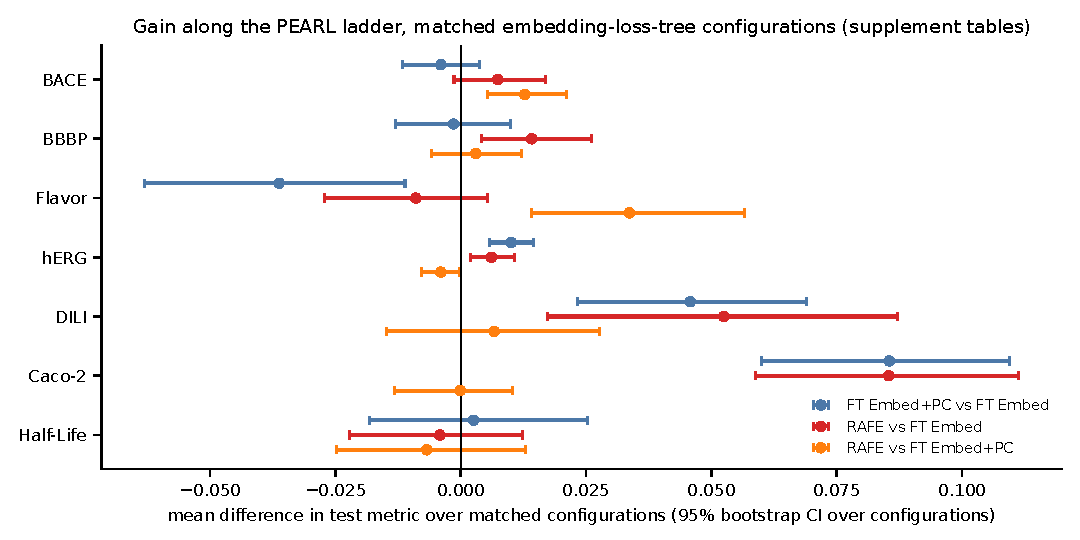
\includegraphics[width=\linewidth,height=0.42\textheight,keepaspectratio]{../results/revision/figures_response/figA_ladder_gain.pdf}
\caption{\textbf{Figure 1.} Difference between pipeline stages over
matched embedding-loss-tree configurations (test metric: MCC for
classification, Spearman correlation for Caco-2 and Half-Life;
supplementary tables; intervals are bootstrap over configurations and
are descriptive because configurations share a test set).}
\end{figure}

\begin{figure}
\centering
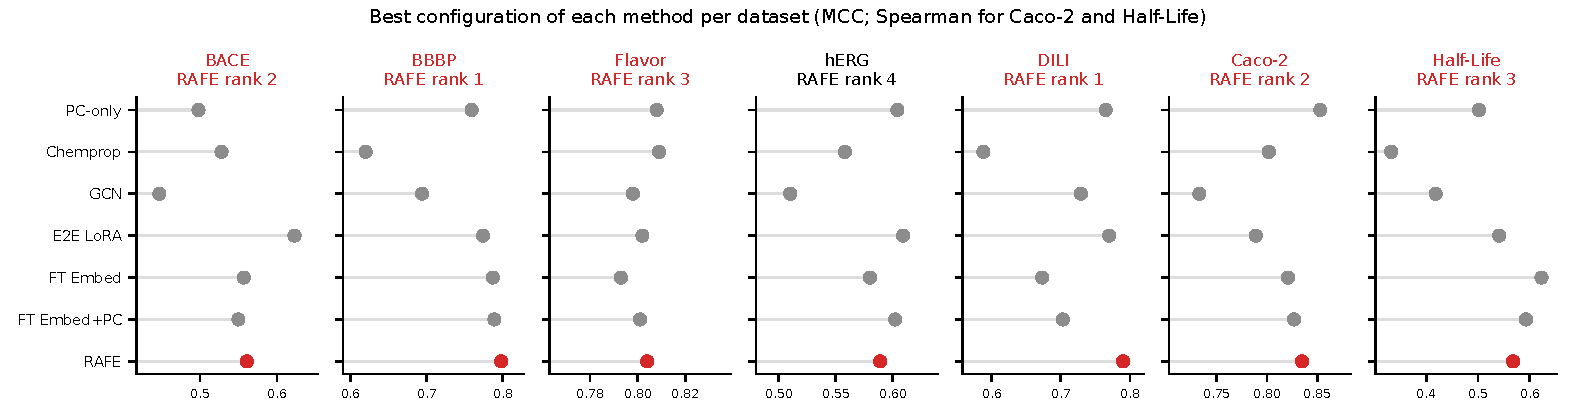
\includegraphics[width=\linewidth,height=0.42\textheight,keepaspectratio]{../results/revision/figures_response/figB_best_config_ranking.pdf}
\caption{\textbf{Figure 2.} Best configuration of each method per
dataset (red: RAFE).}
\end{figure}

\begin{figure}
\centering
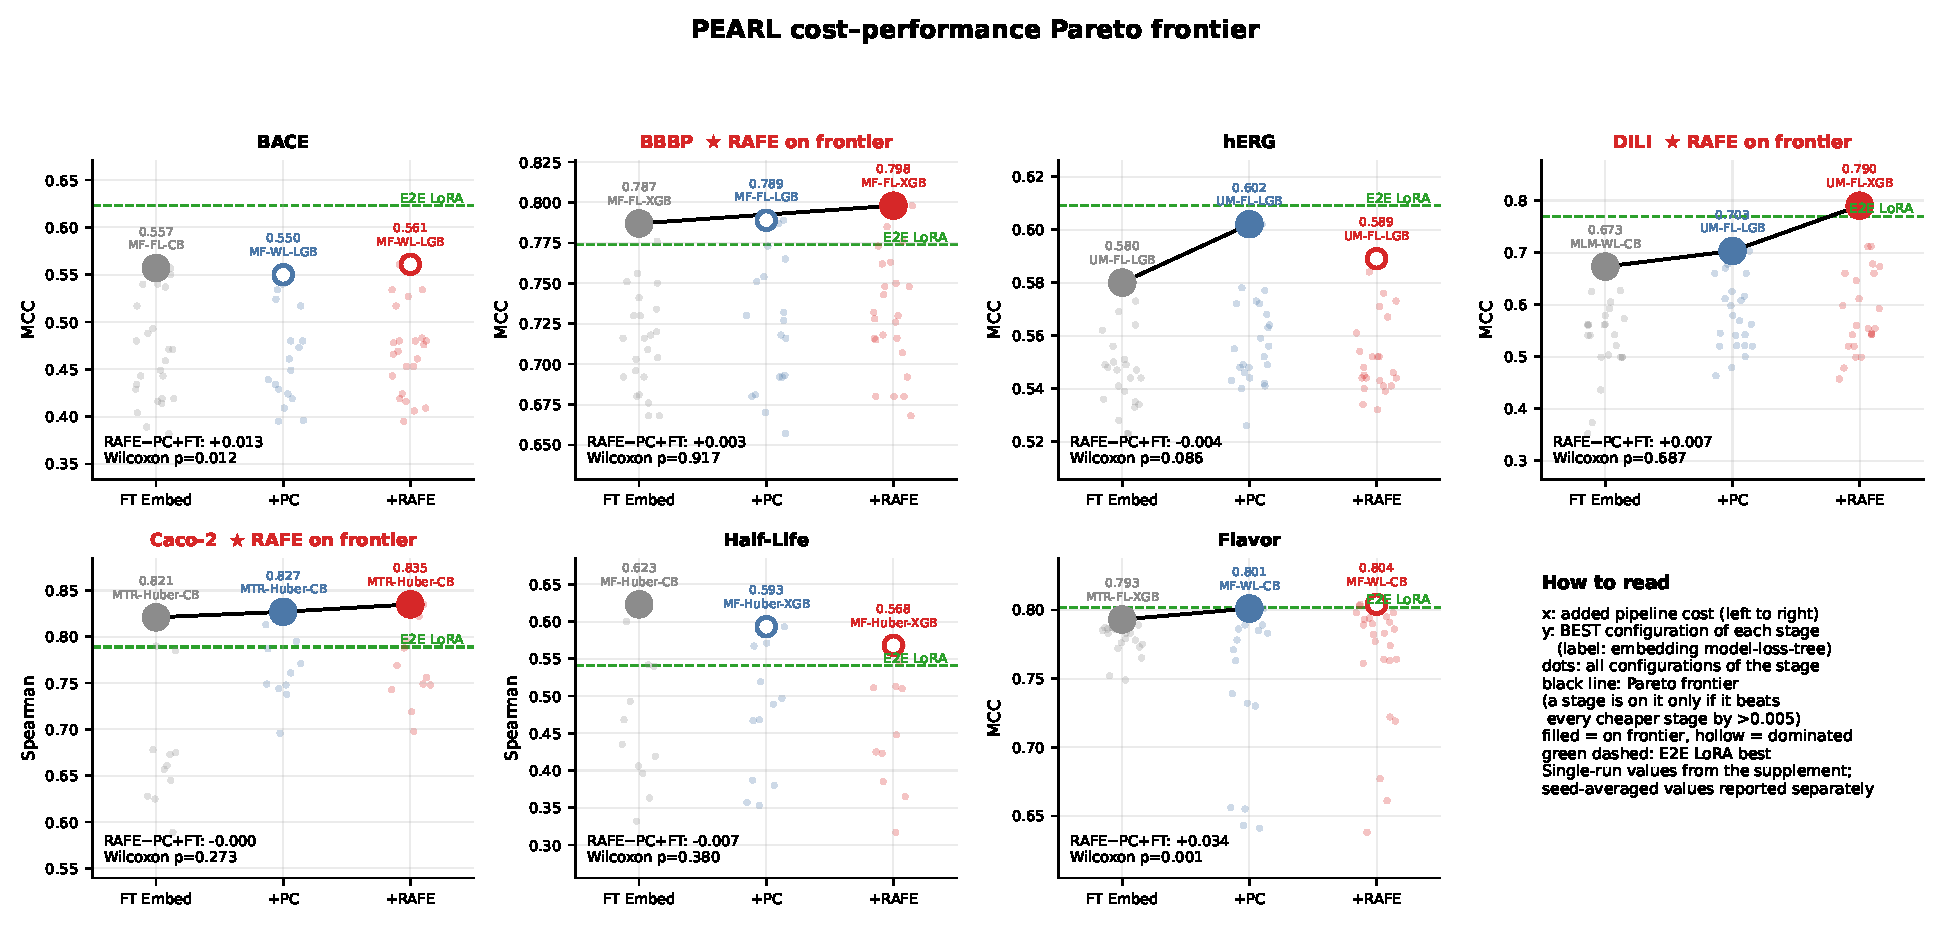
\includegraphics[width=\linewidth,height=0.42\textheight,keepaspectratio]{../results/revision/e12_pareto/pareto_frontier.pdf}
\caption{\textbf{Figure 3.} Cost-performance frontier of the best
configuration of each stage (median view over matched configurations).}
\end{figure}

\textbf{R1.3}

\begin{quote}
Insufficient ablation studies to establish the effectiveness of RAFE.
The authors do not systematically investigate the number of retrieved
neighbors, retrieval similarity metrics, or the individual contributions
of the four RAFE feature groups. Furthermore, different configurations
sometimes employ different downstream tree models, making it difficult
to attribute performance improvements specifically to retrieval
augmentation.
\end{quote}

\textbf{Ans:} We added each control under the identical protocol.

\emph{Feature groups.} Adding or removing any of the four RAFE groups
changes the score by no more than 0.02 in 85\% of the 72 dataset-by-arm
cells (Table 2, Figure 4); the 11 larger shifts are all decreases and
are confined to BACE (test n = 152), DILI (test n = 96), Half-Life (test
n = 133), which have the smallest test sets in the study (n = 96, 133,
152); individual values are listed in Table 2. No single group drives
the effect of RAFE, consistent with the groups carrying overlapping
information (R2.3).

\emph{Retrieval metric and neighbour count.} We compared CLM-cosine
retrieval with Morgan-Tanimoto retrieval and with random retrieval (five
independent random draws), and swept k from 1 to 100. Of 49 paired
comparisons, 2 have an interval that excludes zero (Flavor with
LightGBM, CLM-cosine versus random neighbours (random higher by 0.010):
-0.010, 95\% CI -0.018 to -0.000; Caco-2 with CatBoost, k100 versus k10:
-0.008, 95\% CI -0.015 to -0.001; Figure 5), and both differences are
below 0.011 in size. RAFE therefore needs no tuning of its retrieval
settings. Equal performance of random neighbours shows that it acts as
chemical-space context rather than as an analogue lookup, and the
manuscript now says so. \placeholder{: BBBP neighbour-count sweep
(cells still running)}

\emph{Mixed tree models.} The reviewer is right that the main-text
tables could pair different trees. The controlled matrix (Table 5) and
the full same-tree grids (Tables 5a to 5c) under R2.1 compare every
representation within one tree.

\textbf{Table 2.} RAFE feature-group ablation (5-seed means, each
dataset at its own tree; "+X" adds one group to FT Embed+PC, "RAFE-X"
removes it from full RAFE; A physchem neighbourhood, B density, C
centroid, D Tanimoto).

\begin{longtable}[]{@{}lllllllllll@{}}
\toprule
\begin{minipage}[b]{0.07\columnwidth}\raggedright
Dataset (tree)\strut
\end{minipage} & \begin{minipage}[b]{0.07\columnwidth}\raggedright
FT+PC\strut
\end{minipage} & \begin{minipage}[b]{0.07\columnwidth}\raggedright
+A\strut
\end{minipage} & \begin{minipage}[b]{0.07\columnwidth}\raggedright
+B\strut
\end{minipage} & \begin{minipage}[b]{0.07\columnwidth}\raggedright
+C\strut
\end{minipage} & \begin{minipage}[b]{0.07\columnwidth}\raggedright
+D\strut
\end{minipage} & \begin{minipage}[b]{0.07\columnwidth}\raggedright
RAFE\strut
\end{minipage} & \begin{minipage}[b]{0.07\columnwidth}\raggedright
RAFE-A\strut
\end{minipage} & \begin{minipage}[b]{0.07\columnwidth}\raggedright
RAFE-B\strut
\end{minipage} & \begin{minipage}[b]{0.07\columnwidth}\raggedright
RAFE-C\strut
\end{minipage} & \begin{minipage}[b]{0.07\columnwidth}\raggedright
RAFE-D\strut
\end{minipage}\tabularnewline
\midrule
\endhead
\begin{minipage}[t]{0.07\columnwidth}\raggedright
BBBP (MolFormer-FL) (XGBoost)\strut
\end{minipage} & \begin{minipage}[t]{0.07\columnwidth}\raggedright
0.785\strut
\end{minipage} & \begin{minipage}[t]{0.07\columnwidth}\raggedright
0.790\strut
\end{minipage} & \begin{minipage}[t]{0.07\columnwidth}\raggedright
0.781\strut
\end{minipage} & \begin{minipage}[t]{0.07\columnwidth}\raggedright
0.790\strut
\end{minipage} & \begin{minipage}[t]{0.07\columnwidth}\raggedright
0.780\strut
\end{minipage} & \begin{minipage}[t]{0.07\columnwidth}\raggedright
0.779\strut
\end{minipage} & \begin{minipage}[t]{0.07\columnwidth}\raggedright
0.783\strut
\end{minipage} & \begin{minipage}[t]{0.07\columnwidth}\raggedright
0.779\strut
\end{minipage} & \begin{minipage}[t]{0.07\columnwidth}\raggedright
0.789\strut
\end{minipage} & \begin{minipage}[t]{0.07\columnwidth}\raggedright
0.769\strut
\end{minipage}\tabularnewline
\begin{minipage}[t]{0.07\columnwidth}\raggedright
DILI (Uni-Mol-FL) (XGBoost)\strut
\end{minipage} & \begin{minipage}[t]{0.07\columnwidth}\raggedright
0.693\strut
\end{minipage} & \begin{minipage}[t]{0.07\columnwidth}\raggedright
0.680\strut
\end{minipage} & \begin{minipage}[t]{0.07\columnwidth}\raggedright
0.686\strut
\end{minipage} & \begin{minipage}[t]{0.07\columnwidth}\raggedright
0.673\strut
\end{minipage} & \begin{minipage}[t]{0.07\columnwidth}\raggedright
0.704\strut
\end{minipage} & \begin{minipage}[t]{0.07\columnwidth}\raggedright
0.697\strut
\end{minipage} & \begin{minipage}[t]{0.07\columnwidth}\raggedright
0.671\strut
\end{minipage} & \begin{minipage}[t]{0.07\columnwidth}\raggedright
0.693\strut
\end{minipage} & \begin{minipage}[t]{0.07\columnwidth}\raggedright
0.705\strut
\end{minipage} & \begin{minipage}[t]{0.07\columnwidth}\raggedright
0.651\strut
\end{minipage}\tabularnewline
\begin{minipage}[t]{0.07\columnwidth}\raggedright
Caco-2 (ChemBERTa-MTR) (CatBoost)\strut
\end{minipage} & \begin{minipage}[t]{0.07\columnwidth}\raggedright
0.833\strut
\end{minipage} & \begin{minipage}[t]{0.07\columnwidth}\raggedright
0.826\strut
\end{minipage} & \begin{minipage}[t]{0.07\columnwidth}\raggedright
0.832\strut
\end{minipage} & \begin{minipage}[t]{0.07\columnwidth}\raggedright
0.834\strut
\end{minipage} & \begin{minipage}[t]{0.07\columnwidth}\raggedright
0.835\strut
\end{minipage} & \begin{minipage}[t]{0.07\columnwidth}\raggedright
0.833\strut
\end{minipage} & \begin{minipage}[t]{0.07\columnwidth}\raggedright
0.830\strut
\end{minipage} & \begin{minipage}[t]{0.07\columnwidth}\raggedright
0.835\strut
\end{minipage} & \begin{minipage}[t]{0.07\columnwidth}\raggedright
0.836\strut
\end{minipage} & \begin{minipage}[t]{0.07\columnwidth}\raggedright
0.826\strut
\end{minipage}\tabularnewline
\begin{minipage}[t]{0.07\columnwidth}\raggedright
BACE (MolFormer-WL) (LightGBM)\strut
\end{minipage} & \begin{minipage}[t]{0.07\columnwidth}\raggedright
0.549\strut
\end{minipage} & \begin{minipage}[t]{0.07\columnwidth}\raggedright
0.554\strut
\end{minipage} & \begin{minipage}[t]{0.07\columnwidth}\raggedright
0.553\strut
\end{minipage} & \begin{minipage}[t]{0.07\columnwidth}\raggedright
0.558\strut
\end{minipage} & \begin{minipage}[t]{0.07\columnwidth}\raggedright
0.550\strut
\end{minipage} & \begin{minipage}[t]{0.07\columnwidth}\raggedright
0.553\strut
\end{minipage} & \begin{minipage}[t]{0.07\columnwidth}\raggedright
0.550\strut
\end{minipage} & \begin{minipage}[t]{0.07\columnwidth}\raggedright
0.544\strut
\end{minipage} & \begin{minipage}[t]{0.07\columnwidth}\raggedright
0.548\strut
\end{minipage} & \begin{minipage}[t]{0.07\columnwidth}\raggedright
0.558\strut
\end{minipage}\tabularnewline
\begin{minipage}[t]{0.07\columnwidth}\raggedright
BACE (Uni-Mol-WL) (XGBoost)\strut
\end{minipage} & \begin{minipage}[t]{0.07\columnwidth}\raggedright
0.440\strut
\end{minipage} & \begin{minipage}[t]{0.07\columnwidth}\raggedright
0.455\strut
\end{minipage} & \begin{minipage}[t]{0.07\columnwidth}\raggedright
0.418\strut
\end{minipage} & \begin{minipage}[t]{0.07\columnwidth}\raggedright
0.444\strut
\end{minipage} & \begin{minipage}[t]{0.07\columnwidth}\raggedright
0.433\strut
\end{minipage} & \begin{minipage}[t]{0.07\columnwidth}\raggedright
0.419\strut
\end{minipage} & \begin{minipage}[t]{0.07\columnwidth}\raggedright
0.421\strut
\end{minipage} & \begin{minipage}[t]{0.07\columnwidth}\raggedright
0.433\strut
\end{minipage} & \begin{minipage}[t]{0.07\columnwidth}\raggedright
0.420\strut
\end{minipage} & \begin{minipage}[t]{0.07\columnwidth}\raggedright
0.445\strut
\end{minipage}\tabularnewline
\begin{minipage}[t]{0.07\columnwidth}\raggedright
hERG (MolFormer-FL) (LightGBM)\strut
\end{minipage} & \begin{minipage}[t]{0.07\columnwidth}\raggedright
0.545\strut
\end{minipage} & \begin{minipage}[t]{0.07\columnwidth}\raggedright
0.550\strut
\end{minipage} & \begin{minipage}[t]{0.07\columnwidth}\raggedright
0.544\strut
\end{minipage} & \begin{minipage}[t]{0.07\columnwidth}\raggedright
0.542\strut
\end{minipage} & \begin{minipage}[t]{0.07\columnwidth}\raggedright
0.540\strut
\end{minipage} & \begin{minipage}[t]{0.07\columnwidth}\raggedright
0.544\strut
\end{minipage} & \begin{minipage}[t]{0.07\columnwidth}\raggedright
0.552\strut
\end{minipage} & \begin{minipage}[t]{0.07\columnwidth}\raggedright
0.542\strut
\end{minipage} & \begin{minipage}[t]{0.07\columnwidth}\raggedright
0.545\strut
\end{minipage} & \begin{minipage}[t]{0.07\columnwidth}\raggedright
0.544\strut
\end{minipage}\tabularnewline
\begin{minipage}[t]{0.07\columnwidth}\raggedright
Flavor (MolFormer-WL) (LightGBM)\strut
\end{minipage} & \begin{minipage}[t]{0.07\columnwidth}\raggedright
0.783\strut
\end{minipage} & \begin{minipage}[t]{0.07\columnwidth}\raggedright
0.786\strut
\end{minipage} & \begin{minipage}[t]{0.07\columnwidth}\raggedright
0.785\strut
\end{minipage} & \begin{minipage}[t]{0.07\columnwidth}\raggedright
0.782\strut
\end{minipage} & \begin{minipage}[t]{0.07\columnwidth}\raggedright
0.781\strut
\end{minipage} & \begin{minipage}[t]{0.07\columnwidth}\raggedright
0.785\strut
\end{minipage} & \begin{minipage}[t]{0.07\columnwidth}\raggedright
0.783\strut
\end{minipage} & \begin{minipage}[t]{0.07\columnwidth}\raggedright
0.782\strut
\end{minipage} & \begin{minipage}[t]{0.07\columnwidth}\raggedright
0.783\strut
\end{minipage} & \begin{minipage}[t]{0.07\columnwidth}\raggedright
0.777\strut
\end{minipage}\tabularnewline
\begin{minipage}[t]{0.07\columnwidth}\raggedright
Half-Life (MolFormer) (XGBoost)\strut
\end{minipage} & \begin{minipage}[t]{0.07\columnwidth}\raggedright
0.595\strut
\end{minipage} & \begin{minipage}[t]{0.07\columnwidth}\raggedright
0.571\strut
\end{minipage} & \begin{minipage}[t]{0.07\columnwidth}\raggedright
0.591\strut
\end{minipage} & \begin{minipage}[t]{0.07\columnwidth}\raggedright
0.581\strut
\end{minipage} & \begin{minipage}[t]{0.07\columnwidth}\raggedright
0.593\strut
\end{minipage} & \begin{minipage}[t]{0.07\columnwidth}\raggedright
0.559\strut
\end{minipage} & \begin{minipage}[t]{0.07\columnwidth}\raggedright
0.580\strut
\end{minipage} & \begin{minipage}[t]{0.07\columnwidth}\raggedright
0.565\strut
\end{minipage} & \begin{minipage}[t]{0.07\columnwidth}\raggedright
0.572\strut
\end{minipage} & \begin{minipage}[t]{0.07\columnwidth}\raggedright
0.551\strut
\end{minipage}\tabularnewline
\bottomrule
\end{longtable}

\begin{figure}
\centering
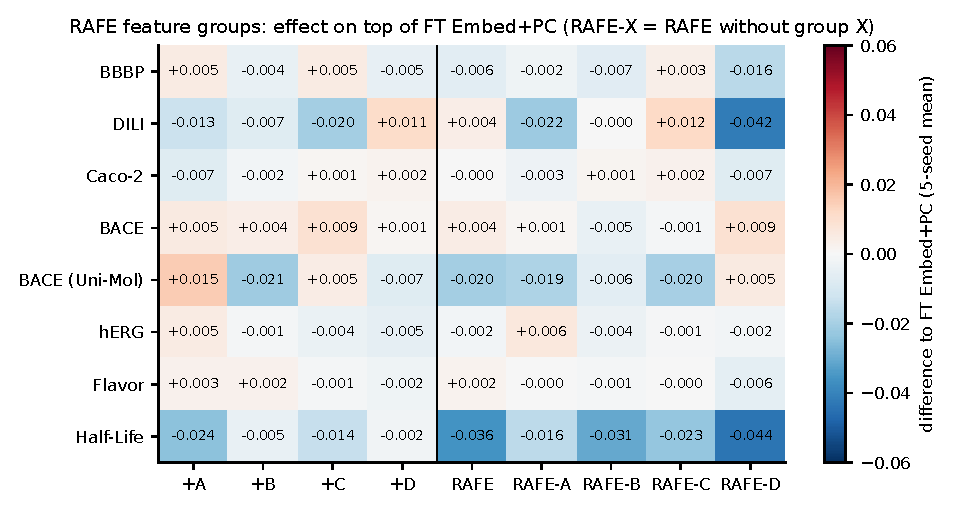
\includegraphics[width=\linewidth,height=0.42\textheight,keepaspectratio]{../results/revision/figures_response/figC_ablation_heatmap.pdf}
\caption{\textbf{Figure 4.} Change relative to FT Embed+PC for each
feature-group arm (RAFE-X: RAFE without group X).}
\end{figure}

\begin{figure}
\centering
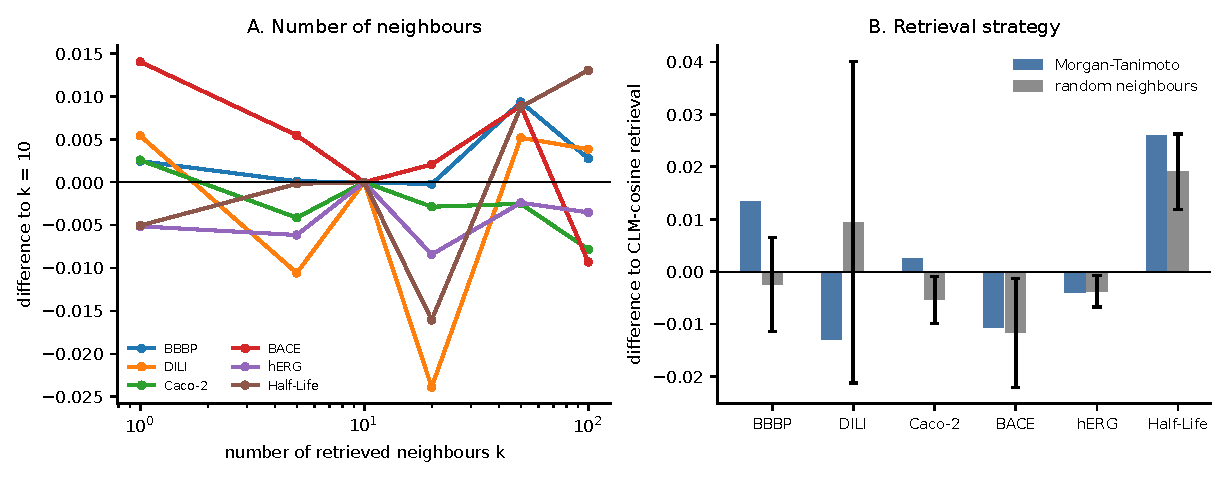
\includegraphics[width=\linewidth,height=0.42\textheight,keepaspectratio]{../results/revision/figures_response/figD_retrieval_robustness.pdf}
\caption{\textbf{Figure 5.} Left: effect of the number of retrieved
neighbours (difference to k = 10). Right: effect of the retrieval
strategy (difference to CLM-cosine retrieval; error bars: spread over
the five random draws).}
\end{figure}

\textbf{R1.4}

\begin{quote}
Adequacy of the ZINC-250k Retrieval Database: The authors use ZINC-250k,
containing approximately 250,000 molecules, as the retrieval database.
However, it remains unclear whether this dataset provides sufficient
coverage of the diverse chemical spaces represented by the downstream
tasks.
\end{quote}

\textbf{Ans:} We measured, for every dataset molecule, the largest
Morgan-Tanimoto similarity to ZINC-250k (Table 3, Figure 6). The median
is 0.40 over all 34,018 molecules, and about 5\% have a neighbour at 0.6
or above; BACE is the least covered (median 0.338). ZINC-250k therefore
provides background chemical context rather than close analogues.
Consistent with this, the per-molecule gain from RAFE is unrelated to
coverage (R2.3) and random neighbours perform like similar ones (R1.3).
Whether a task-matched library would do better is untested and is listed
as a limitation. {[}Revision{]}

\textbf{Table 3.} Coverage of the dataset molecules by ZINC-250k.

\begin{longtable}[]{@{}llllll@{}}
\toprule
\begin{minipage}[b]{0.14\columnwidth}\raggedright
Dataset\strut
\end{minipage} & \begin{minipage}[b]{0.14\columnwidth}\raggedright
Molecules\strut
\end{minipage} & \begin{minipage}[b]{0.14\columnwidth}\raggedright
Median max Tanimoto to ZINC\strut
\end{minipage} & \begin{minipage}[b]{0.14\columnwidth}\raggedright
Fraction \textgreater=0.4\strut
\end{minipage} & \begin{minipage}[b]{0.14\columnwidth}\raggedright
Fraction \textgreater=0.6\strut
\end{minipage} & \begin{minipage}[b]{0.14\columnwidth}\raggedright
Fraction \textgreater=0.8\strut
\end{minipage}\tabularnewline
\midrule
\endhead
\begin{minipage}[t]{0.14\columnwidth}\raggedright
BACE\strut
\end{minipage} & \begin{minipage}[t]{0.14\columnwidth}\raggedright
1513\strut
\end{minipage} & \begin{minipage}[t]{0.14\columnwidth}\raggedright
0.338\strut
\end{minipage} & \begin{minipage}[t]{0.14\columnwidth}\raggedright
0.151\strut
\end{minipage} & \begin{minipage}[t]{0.14\columnwidth}\raggedright
0.002\strut
\end{minipage} & \begin{minipage}[t]{0.14\columnwidth}\raggedright
0.000\strut
\end{minipage}\tabularnewline
\begin{minipage}[t]{0.14\columnwidth}\raggedright
BBBP\strut
\end{minipage} & \begin{minipage}[t]{0.14\columnwidth}\raggedright
1996\strut
\end{minipage} & \begin{minipage}[t]{0.14\columnwidth}\raggedright
0.418\strut
\end{minipage} & \begin{minipage}[t]{0.14\columnwidth}\raggedright
0.581\strut
\end{minipage} & \begin{minipage}[t]{0.14\columnwidth}\raggedright
0.128\strut
\end{minipage} & \begin{minipage}[t]{0.14\columnwidth}\raggedright
0.021\strut
\end{minipage}\tabularnewline
\begin{minipage}[t]{0.14\columnwidth}\raggedright
Caco-2\strut
\end{minipage} & \begin{minipage}[t]{0.14\columnwidth}\raggedright
910\strut
\end{minipage} & \begin{minipage}[t]{0.14\columnwidth}\raggedright
0.404\strut
\end{minipage} & \begin{minipage}[t]{0.14\columnwidth}\raggedright
0.526\strut
\end{minipage} & \begin{minipage}[t]{0.14\columnwidth}\raggedright
0.080\strut
\end{minipage} & \begin{minipage}[t]{0.14\columnwidth}\raggedright
0.008\strut
\end{minipage}\tabularnewline
\begin{minipage}[t]{0.14\columnwidth}\raggedright
DILI\strut
\end{minipage} & \begin{minipage}[t]{0.14\columnwidth}\raggedright
475\strut
\end{minipage} & \begin{minipage}[t]{0.14\columnwidth}\raggedright
0.425\strut
\end{minipage} & \begin{minipage}[t]{0.14\columnwidth}\raggedright
0.587\strut
\end{minipage} & \begin{minipage}[t]{0.14\columnwidth}\raggedright
0.135\strut
\end{minipage} & \begin{minipage}[t]{0.14\columnwidth}\raggedright
0.013\strut
\end{minipage}\tabularnewline
\begin{minipage}[t]{0.14\columnwidth}\raggedright
Flavor\strut
\end{minipage} & \begin{minipage}[t]{0.14\columnwidth}\raggedright
15025\strut
\end{minipage} & \begin{minipage}[t]{0.14\columnwidth}\raggedright
0.431\strut
\end{minipage} & \begin{minipage}[t]{0.14\columnwidth}\raggedright
0.624\strut
\end{minipage} & \begin{minipage}[t]{0.14\columnwidth}\raggedright
0.070\strut
\end{minipage} & \begin{minipage}[t]{0.14\columnwidth}\raggedright
0.006\strut
\end{minipage}\tabularnewline
\begin{minipage}[t]{0.14\columnwidth}\raggedright
Half-Life\strut
\end{minipage} & \begin{minipage}[t]{0.14\columnwidth}\raggedright
654\strut
\end{minipage} & \begin{minipage}[t]{0.14\columnwidth}\raggedright
0.407\strut
\end{minipage} & \begin{minipage}[t]{0.14\columnwidth}\raggedright
0.526\strut
\end{minipage} & \begin{minipage}[t]{0.14\columnwidth}\raggedright
0.104\strut
\end{minipage} & \begin{minipage}[t]{0.14\columnwidth}\raggedright
0.015\strut
\end{minipage}\tabularnewline
\begin{minipage}[t]{0.14\columnwidth}\raggedright
hERG\strut
\end{minipage} & \begin{minipage}[t]{0.14\columnwidth}\raggedright
13445\strut
\end{minipage} & \begin{minipage}[t]{0.14\columnwidth}\raggedright
0.375\strut
\end{minipage} & \begin{minipage}[t]{0.14\columnwidth}\raggedright
0.382\strut
\end{minipage} & \begin{minipage}[t]{0.14\columnwidth}\raggedright
0.016\strut
\end{minipage} & \begin{minipage}[t]{0.14\columnwidth}\raggedright
0.001\strut
\end{minipage}\tabularnewline
\bottomrule
\end{longtable}

\begin{figure}
\centering
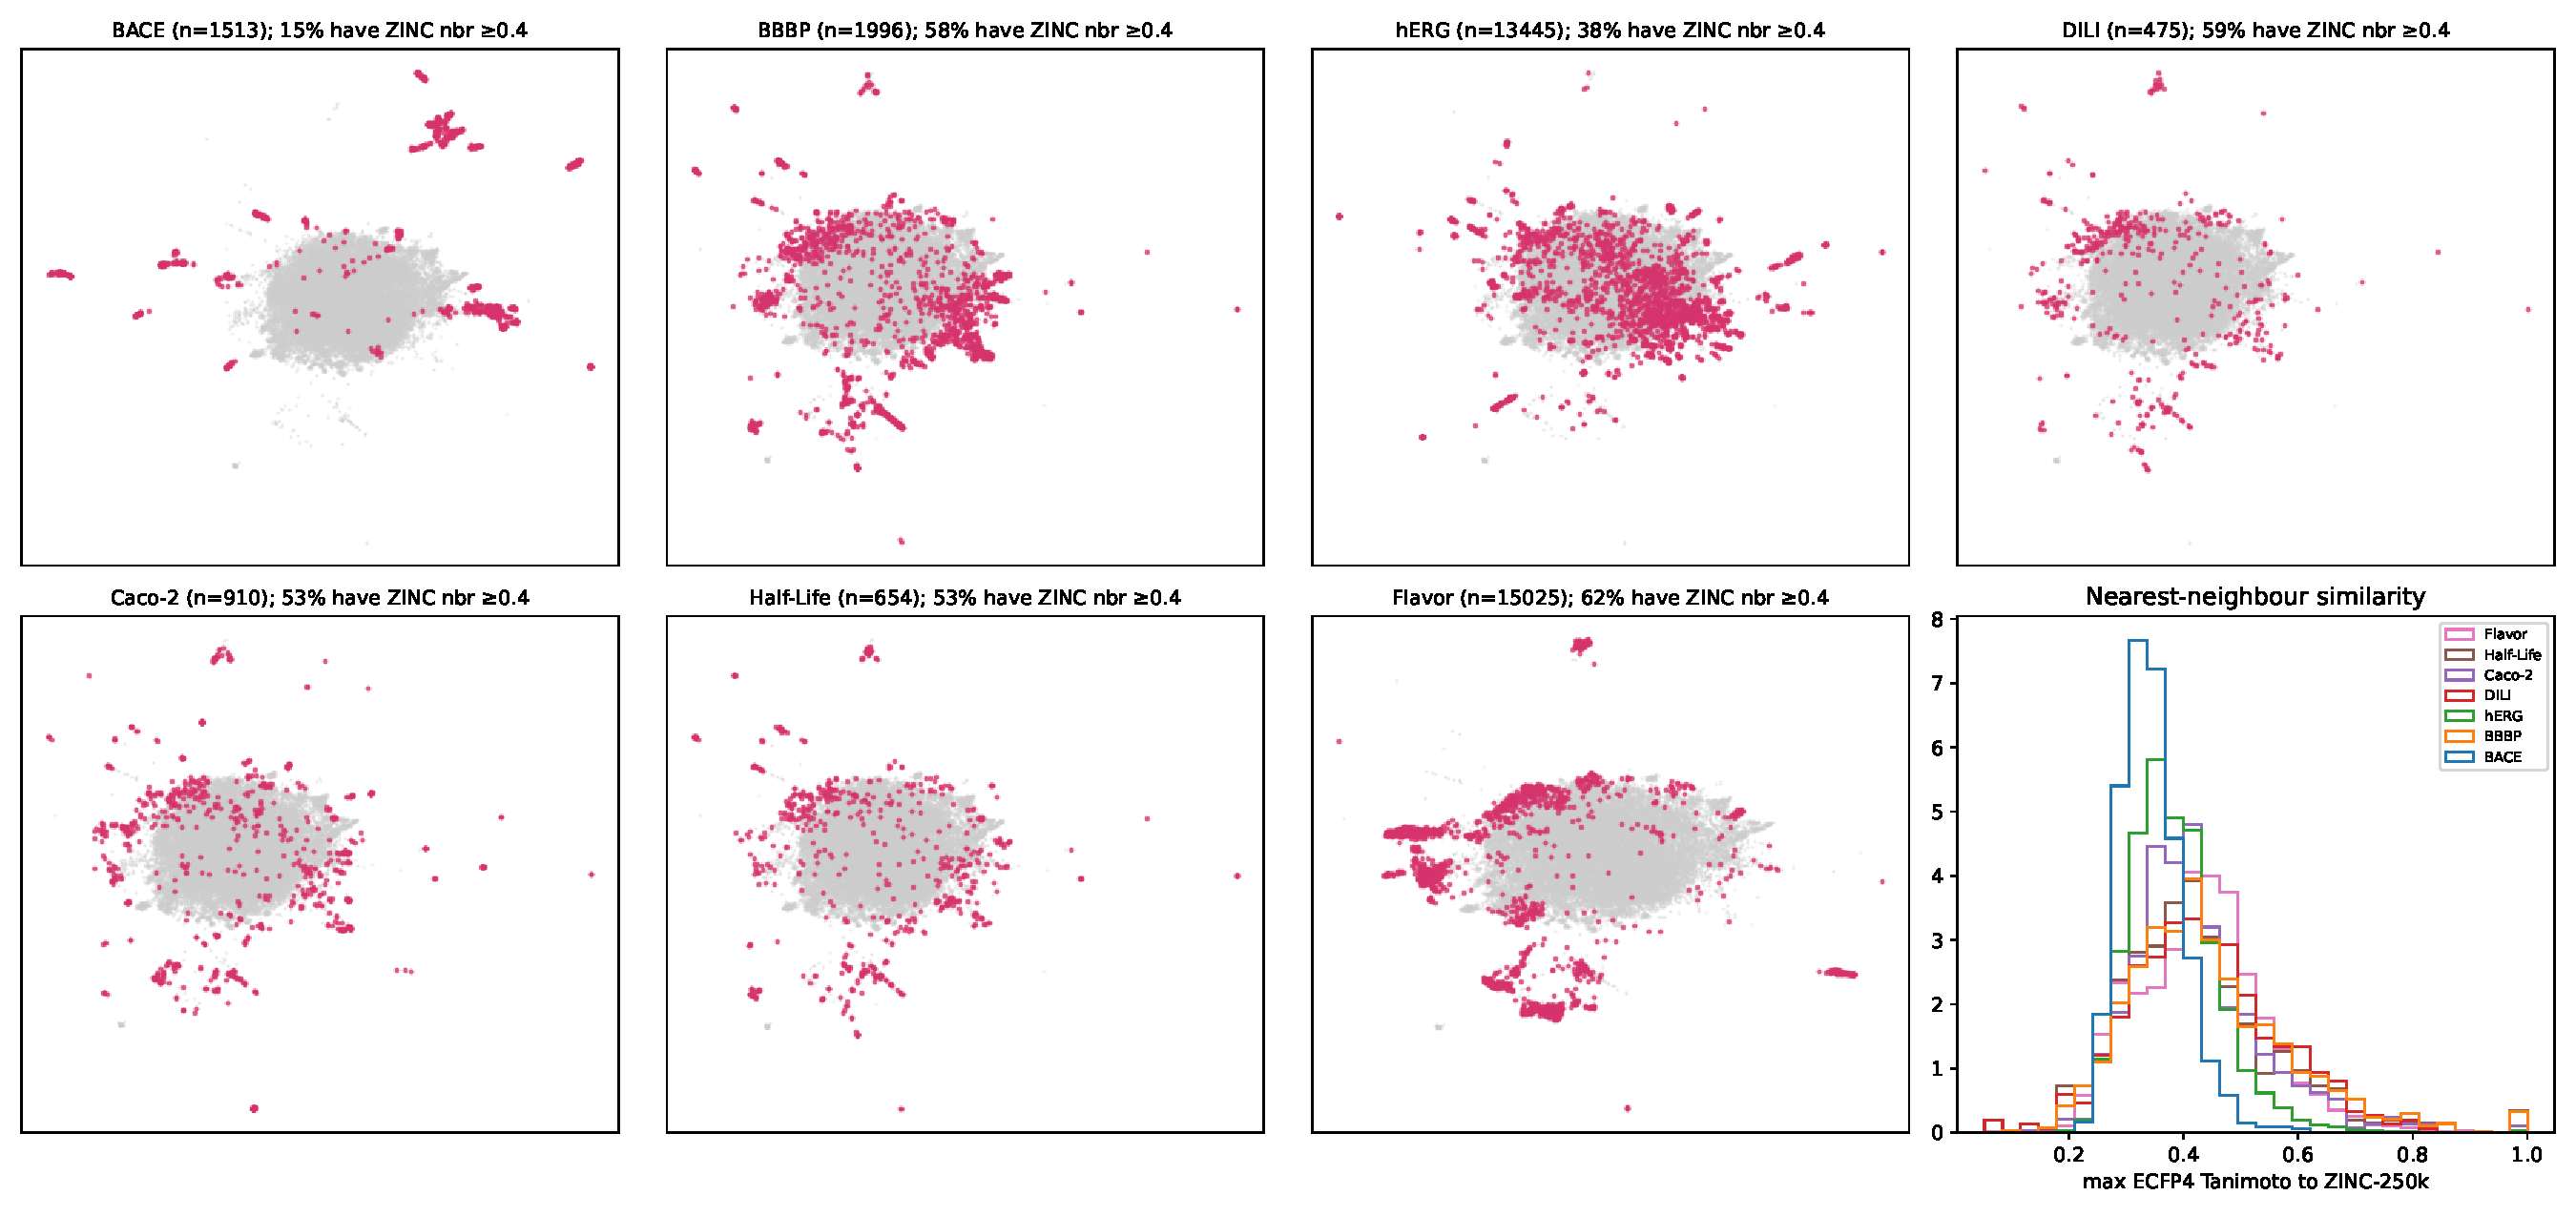
\includegraphics[width=\linewidth,height=0.42\textheight,keepaspectratio]{../results/revision/e07_coverage/umap_coverage.pdf}
\caption{\textbf{Figure 6.} Joint UMAP of the dataset molecules and
ZINC-250k.}
\end{figure}

\textbf{R1.5}

\begin{quote}
End-to-End Computational Efficiency and Runtime Analysis: Although the
paper emphasizes parameter efficiency through LoRA and reports low FAISS
retrieval latency, it lacks a comprehensive evaluation of the
computational cost of the entire PEARL pipeline.
\end{quote}

\textbf{Ans:} Table 4 and Figure 7 give the cost of each stage, measured
or taken from the logs of the original runs (no cross-method comparison,
as discussed). One-off costs are small for the SMILES models (LoRA
fine-tuning in seconds to minutes; embedding the 249k-molecule library
in about 4.3 minutes) and large for Uni-Mol (hours, dominated by
conformer generation). At prediction time RAFE adds about 0.13 s per
molecule on a shared GPU, using exact search; tree inference takes under
a millisecond. The figures come from different hardware and are
indicative. {[}Revision: new subsection "Computational cost"{]}

\textbf{Table 4.} Runtime of the pipeline stages.

\begin{longtable}[]{@{}lll@{}}
\toprule
\begin{minipage}[b]{0.30\columnwidth}\raggedright
Stage\strut
\end{minipage} & \begin{minipage}[b]{0.30\columnwidth}\raggedright
Cost\strut
\end{minipage} & \begin{minipage}[b]{0.30\columnwidth}\raggedright
Source\strut
\end{minipage}\tabularnewline
\midrule
\endhead
\begin{minipage}[t]{0.30\columnwidth}\raggedright
LoRA fine-tuning, one run\strut
\end{minipage} & \begin{minipage}[t]{0.30\columnwidth}\raggedright
median 13 s, IQR 6-43 s, max 540 s\strut
\end{minipage} & \begin{minipage}[t]{0.30\columnwidth}\raggedright
training logs; includes small test runs, so a lower bound per
dataset\strut
\end{minipage}\tabularnewline
\begin{minipage}[t]{0.30\columnwidth}\raggedright
Library embedding, SMILES models (6 variants)\strut
\end{minipage} & \begin{minipage}[t]{0.30\columnwidth}\raggedright
4.4 min (hERG), 4.2 min (DILI)\strut
\end{minipage} & \begin{minipage}[t]{0.30\columnwidth}\raggedright
original run logs\strut
\end{minipage}\tabularnewline
\begin{minipage}[t]{0.30\columnwidth}\raggedright
Library embedding, Uni-Mol\strut
\end{minipage} & \begin{minipage}[t]{0.30\columnwidth}\raggedright
herg: 8.4 h, dili: 9.1 h, caco2: 1.7 h (hERG and DILI: 2 variants each;
Caco-2 rerun: 1 variant)\strut
\end{minipage} & \begin{minipage}[t]{0.30\columnwidth}\raggedright
original run logs\strut
\end{minipage}\tabularnewline
\begin{minipage}[t]{0.30\columnwidth}\raggedright
RAFE at inference, one molecule\strut
\end{minipage} & \begin{minipage}[t]{0.30\columnwidth}\raggedright
retrieval 125.8 ms, features 3.8 ms, total 129.6 ms (129.63 ms per
molecule)\strut
\end{minipage} & \begin{minipage}[t]{0.30\columnwidth}\raggedright
measured, shared P100, exact search over 249k molecules\strut
\end{minipage}\tabularnewline
\begin{minipage}[t]{0.30\columnwidth}\raggedright
RAFE at inference, 192 molecules\strut
\end{minipage} & \begin{minipage}[t]{0.30\columnwidth}\raggedright
retrieval 139.8 ms, features 456.2 ms, total 596.0 ms (3.10 ms per
molecule)\strut
\end{minipage} & \begin{minipage}[t]{0.30\columnwidth}\raggedright
measured\strut
\end{minipage}\tabularnewline
\begin{minipage}[t]{0.30\columnwidth}\raggedright
XGBoost inference, one molecule\strut
\end{minipage} & \begin{minipage}[t]{0.30\columnwidth}\raggedright
0.5 ms\strut
\end{minipage} & \begin{minipage}[t]{0.30\columnwidth}\raggedright
measured\strut
\end{minipage}\tabularnewline
\begin{minipage}[t]{0.30\columnwidth}\raggedright
Tree stage per cell (20 Optuna trials × 5-fold CV + fit)\strut
\end{minipage} & \begin{minipage}[t]{0.30\columnwidth}\raggedright
XGBoost median 639 s, IQR 398-888 s; LightGBM median 213 s, IQR 33-778
s; CatBoost median 1560 s, IQR 833-4380 s\strut
\end{minipage} & \begin{minipage}[t]{0.30\columnwidth}\raggedright
E1 and E4 cells on a loaded shared server; an upper bound\strut
\end{minipage}\tabularnewline
\bottomrule
\end{longtable}

\begin{figure}
\centering
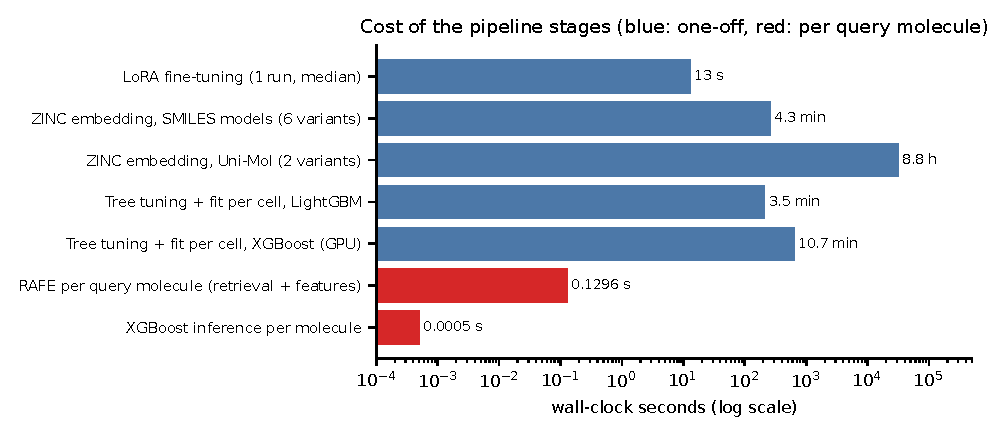
\includegraphics[width=\linewidth,height=0.42\textheight,keepaspectratio]{../results/revision/figures_response/figE_runtime.pdf}
\caption{\textbf{Figure 7.} Cost of the pipeline stages (blue: one-off;
red: per query molecule).}
\end{figure}

\begin{center}\rule{0.5\linewidth}{0.5pt}\end{center}

\hypertarget{reviewer-2}{%
\subsection{Reviewer 2}\label{reviewer-2}}

\textbf{R2.1}

\begin{quote}
Lack of controlled comparisons between molecular representations and
machine learning algorithms. This is my primary concern with the
manuscript. The authors evaluate different feature representations using
XGBoost, LightGBM, and CatBoost. However, Tables 2 and 3 present
selected best-performing configurations rather than a complete,
controlled comparison in which the same prediction algorithm is applied
to every representation. For example, in Table 2, RAFE is evaluated
using XGBoost, whereas FT Embed + PC is represented by LightGBM.
Therefore, the reported performance difference cannot be attributed
exclusively to the inclusion of retrieval-augmented features. A similar
issue arises from the selection of different prediction algorithms
across experimental configurations. Selecting the best combination for
each representation may be appropriate for comparing optimized
prediction pipelines, but it does not establish the independent
contribution of the proposed representation. A fundamental experiment is
needed in which all representations are evaluated using the same
downstream prediction algorithms, data partitions, and comparable
hyperparameter optimization budgets. At minimum, the comparisons should
include PC-only, FT Embed, FT Embed + PC, and RAFE, each evaluated
independently using XGBoost, LightGBM, and CatBoost. Without this
controlled experimental design, it is difficult to determine whether the
reported improvements originate from RAFE or from the choice of
prediction algorithm and its optimization.
\end{quote}

\textbf{Ans:} We thank the reviewer for pressing on this; it is the
comment that shaped the revision. The main-text tables reported the best
row per representation, which is not a controlled comparison. We have
now run PC-only, FT Embed, FT Embed+PC and RAFE through the same code,
splits and test molecules, with the same tuning budget (20 Optuna
trials, 5-fold cross-validation on the training split only), the same
three tree models and the same five seeds (Table 5, Figure 8). The test
split is evaluated once per fitted model. {[}Revision: Methods, and a
main-text table with the full matrix in the supplement{]}

The outcome is clear. RAFE is never significantly different from FT
Embed+PC (24 paired comparisons: 0 better, 0 worse), so the final stage
carries no detectable cost. It is significantly better than the
fine-tuned embedding alone in 5 of 24 comparisons (Caco-2, DILI, hERG)
and never worse. Which stage wins depends on the dataset: the embedding
helps over descriptors on BACE (MolFormer), BBBP and Half-Life, whereas
PC-only is strongest or tied on Caco-2, hERG and Flavor, and RAFE is
significantly below PC-only in 4 of 24 comparisons (Flavor, hERG) and
significantly above it in 0. Identifying such dataset-specific winners
is the purpose of the benchmark.

\textbf{Table 5.} Controlled comparison (mean over seeds; MCC for
classification, Spearman for regression; one embedding configuration per
dataset).

\begin{longtable}[]{@{}lllllll@{}}
\toprule
Dataset (embedding) & Metric & Tree & PC-only & FT Embed & FT Embed+PC &
RAFE\tabularnewline
\midrule
\endhead
BACE (MolFormer-WL) & MCC & CatBoost & 0.465 & 0.546 & 0.528 &
0.518\tabularnewline
BACE (MolFormer-WL) & MCC & LightGBM & 0.485 & 0.539 & 0.549 &
0.553\tabularnewline
BACE (MolFormer-WL) & MCC & XGBoost & 0.477 & 0.542 & 0.538 &
0.527\tabularnewline
BACE (Uni-Mol-WL) & MCC & CatBoost & 0.465 & 0.390 & 0.440 &
0.425\tabularnewline
BACE (Uni-Mol-WL) & MCC & LightGBM & 0.485 & 0.421 & 0.439 &
0.424\tabularnewline
BACE (Uni-Mol-WL) & MCC & XGBoost & 0.477 & 0.429 & 0.440 &
0.419\tabularnewline
BBBP (MolFormer-FL) & MCC & CatBoost & 0.726 & 0.762 & 0.768 &
0.799\tabularnewline
BBBP (MolFormer-FL) & MCC & LightGBM & 0.733 & 0.768 & 0.755 &
0.767\tabularnewline
BBBP (MolFormer-FL) & MCC & XGBoost & 0.731 & 0.783 & 0.785 &
0.779\tabularnewline
Caco-2 (ChemBERTa-MTR) & Spearman & CatBoost & 0.840 & 0.809 & 0.833 &
0.833\tabularnewline
Caco-2 (ChemBERTa-MTR) & Spearman & LightGBM & 0.834 & 0.789 & 0.819 &
0.816\tabularnewline
Caco-2 (ChemBERTa-MTR) & Spearman & XGBoost & 0.833 & 0.788 & 0.813 &
0.817\tabularnewline
DILI (Uni-Mol-FL) & MCC & CatBoost & 0.738 & 0.595 & 0.683 &
0.669\tabularnewline
DILI (Uni-Mol-FL) & MCC & LightGBM & 0.654 & 0.574 & 0.690 &
0.658\tabularnewline
DILI (Uni-Mol-FL) & MCC & XGBoost & 0.672 & 0.520 & 0.693 &
0.697\tabularnewline
Flavor (MolFormer-WL) & MCC & CatBoost & 0.798 & 0.789 & 0.789 &
0.786\tabularnewline
Flavor (MolFormer-WL) & MCC & LightGBM & 0.798 & 0.779 & 0.783 &
0.785\tabularnewline
Flavor (MolFormer-WL) & MCC & XGBoost & 0.809 & 0.782 & 0.780 &
0.782\tabularnewline
Half-Life (MolFormer) & Spearman & CatBoost & 0.530 & 0.604 & 0.596 &
0.577\tabularnewline
Half-Life (MolFormer) & Spearman & LightGBM & 0.477 & 0.550 & 0.558 &
0.512\tabularnewline
Half-Life (MolFormer) & Spearman & XGBoost & 0.499 & 0.592 & 0.595 &
0.559\tabularnewline
hERG (MolFormer-FL) & MCC & CatBoost & 0.593 & 0.536 & 0.543 &
0.537\tabularnewline
hERG (MolFormer-FL) & MCC & LightGBM & 0.577 & 0.532 & 0.545 &
0.544\tabularnewline
hERG (MolFormer-FL) & MCC & XGBoost & 0.594 & 0.545 & 0.546 &
0.545\tabularnewline
\bottomrule
\end{longtable}

\begin{figure}
\centering
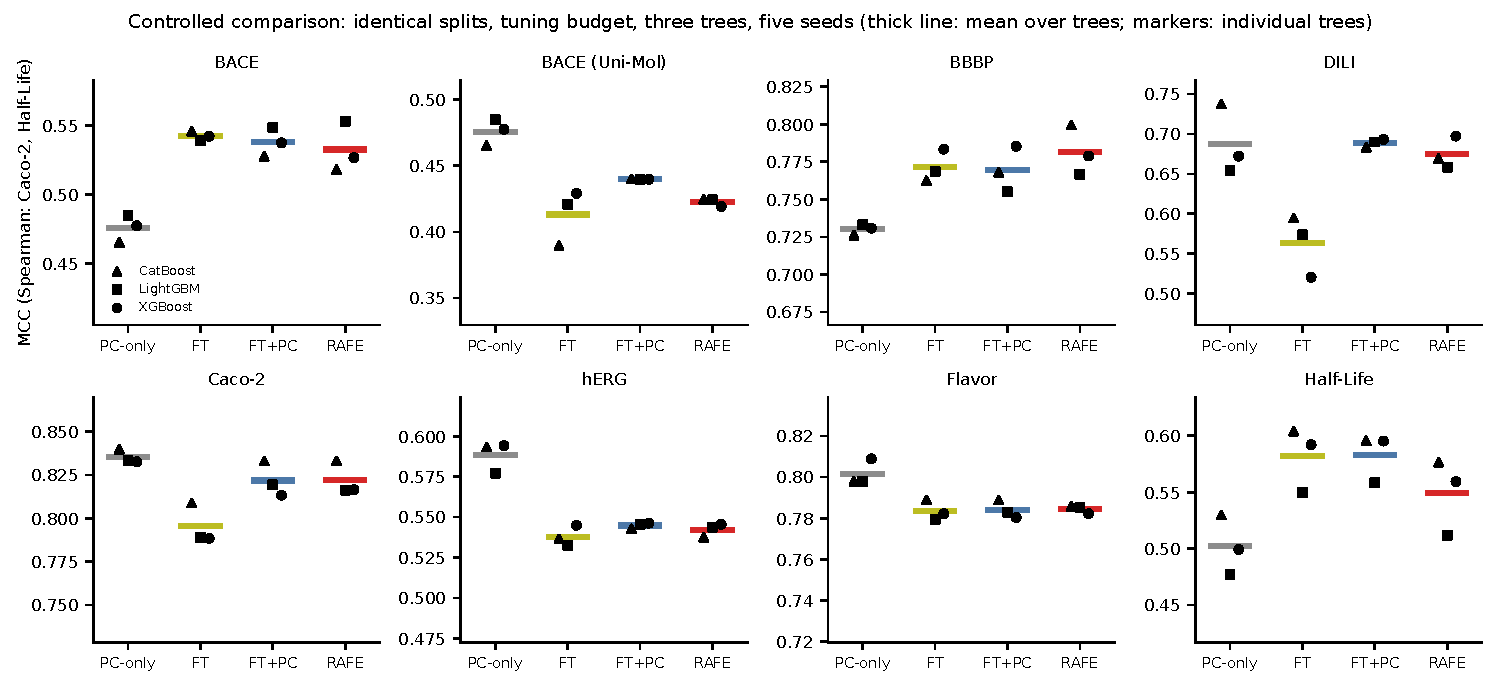
\includegraphics[width=\linewidth,height=0.42\textheight,keepaspectratio]{../results/revision/figures_response/figF_controlled_matrix.pdf}
\caption{\textbf{Figure 8.} The controlled comparison of Table 5 (thick
line: mean over trees; markers: individual trees).}
\end{figure}

Because the reviewer's concern is that best rows may pair different
trees, we also give the full grid for the three datasets where RAFE
matters most (Tables 5a to 5c: every embedding and loss, compared within
one tree; the bottom rows pool the difference over rows and seeds with
paired intervals). On DILI, RAFE exceeds FT Embed with both trees, and
exceeds FT Embed+PC with XGBoost (+0.032, interval +0.005 to +0.060) but
not with LightGBM (-0.009, -0.029 to +0.012). On Caco-2, RAFE and FT
Embed+PC are indistinguishable and both exceed FT Embed by about 0.08,
while PC-only is above every stage. On BBBP no stage separates from
another. On Half-Life RAFE falls below FT Embed+PC with LightGBM
(-0.023, -0.044 to -0.002). CatBoost columns are still running.
\placeholder{: CatBoost columns of Tables 5a to 5c}

\textbf{Table 5a.} \textbf{DILI}: mean ± SD test MCC over five seeds (42
to 46). Bold: best of the three stages within the row and tree.

\begin{longtable}[]{@{}lllllll@{}}
\toprule
\begin{minipage}[b]{0.12\columnwidth}\raggedright
Embedding, loss\strut
\end{minipage} & \begin{minipage}[b]{0.12\columnwidth}\raggedright
XGBoost: FT Embed\strut
\end{minipage} & \begin{minipage}[b]{0.12\columnwidth}\raggedright
XGBoost: FT Embed+PC\strut
\end{minipage} & \begin{minipage}[b]{0.12\columnwidth}\raggedright
XGBoost: RAFE\strut
\end{minipage} & \begin{minipage}[b]{0.12\columnwidth}\raggedright
LightGBM: FT Embed\strut
\end{minipage} & \begin{minipage}[b]{0.12\columnwidth}\raggedright
LightGBM: FT Embed+PC\strut
\end{minipage} & \begin{minipage}[b]{0.12\columnwidth}\raggedright
LightGBM: RAFE\strut
\end{minipage}\tabularnewline
\midrule
\endhead
\begin{minipage}[t]{0.12\columnwidth}\raggedright
ChemBERTa-MLM FL\strut
\end{minipage} & \begin{minipage}[t]{0.12\columnwidth}\raggedright
0.536 ± 0.025\strut
\end{minipage} & \begin{minipage}[t]{0.12\columnwidth}\raggedright
0.522 ± 0.020\strut
\end{minipage} & \begin{minipage}[t]{0.12\columnwidth}\raggedright
\textbf{0.637 ± 0.024}\strut
\end{minipage} & \begin{minipage}[t]{0.12\columnwidth}\raggedright
0.613 ± 0.047\strut
\end{minipage} & \begin{minipage}[t]{0.12\columnwidth}\raggedright
\textbf{0.645 ± 0.039}\strut
\end{minipage} & \begin{minipage}[t]{0.12\columnwidth}\raggedright
0.617 ± 0.060\strut
\end{minipage}\tabularnewline
\begin{minipage}[t]{0.12\columnwidth}\raggedright
ChemBERTa-MLM WL\strut
\end{minipage} & \begin{minipage}[t]{0.12\columnwidth}\raggedright
0.563 ± 0.059\strut
\end{minipage} & \begin{minipage}[t]{0.12\columnwidth}\raggedright
0.542 ± 0.057\strut
\end{minipage} & \begin{minipage}[t]{0.12\columnwidth}\raggedright
\textbf{0.565 ± 0.024}\strut
\end{minipage} & \begin{minipage}[t]{0.12\columnwidth}\raggedright
\textbf{0.579 ± 0.021}\strut
\end{minipage} & \begin{minipage}[t]{0.12\columnwidth}\raggedright
0.574 ± 0.030\strut
\end{minipage} & \begin{minipage}[t]{0.12\columnwidth}\raggedright
0.564 ± 0.021\strut
\end{minipage}\tabularnewline
\begin{minipage}[t]{0.12\columnwidth}\raggedright
ChemBERTa-MTR FL\strut
\end{minipage} & \begin{minipage}[t]{0.12\columnwidth}\raggedright
0.412 ± 0.046\strut
\end{minipage} & \begin{minipage}[t]{0.12\columnwidth}\raggedright
0.467 ± 0.030\strut
\end{minipage} & \begin{minipage}[t]{0.12\columnwidth}\raggedright
\textbf{0.543 ± 0.040}\strut
\end{minipage} & \begin{minipage}[t]{0.12\columnwidth}\raggedright
0.416 ± 0.021\strut
\end{minipage} & \begin{minipage}[t]{0.12\columnwidth}\raggedright
0.521 ± 0.025\strut
\end{minipage} & \begin{minipage}[t]{0.12\columnwidth}\raggedright
\textbf{0.535 ± 0.052}\strut
\end{minipage}\tabularnewline
\begin{minipage}[t]{0.12\columnwidth}\raggedright
ChemBERTa-MTR WL\strut
\end{minipage} & \begin{minipage}[t]{0.12\columnwidth}\raggedright
0.546 ± 0.026\strut
\end{minipage} & \begin{minipage}[t]{0.12\columnwidth}\raggedright
0.542 ± 0.028\strut
\end{minipage} & \begin{minipage}[t]{0.12\columnwidth}\raggedright
\textbf{0.562 ± 0.025}\strut
\end{minipage} & \begin{minipage}[t]{0.12\columnwidth}\raggedright
\textbf{0.558 ± 0.017}\strut
\end{minipage} & \begin{minipage}[t]{0.12\columnwidth}\raggedright
0.534 ± 0.025\strut
\end{minipage} & \begin{minipage}[t]{0.12\columnwidth}\raggedright
0.538 ± 0.031\strut
\end{minipage}\tabularnewline
\begin{minipage}[t]{0.12\columnwidth}\raggedright
MolFormer FL\strut
\end{minipage} & \begin{minipage}[t]{0.12\columnwidth}\raggedright
0.507 ± 0.038\strut
\end{minipage} & \begin{minipage}[t]{0.12\columnwidth}\raggedright
0.537 ± 0.018\strut
\end{minipage} & \begin{minipage}[t]{0.12\columnwidth}\raggedright
\textbf{0.541 ± 0.021}\strut
\end{minipage} & \begin{minipage}[t]{0.12\columnwidth}\raggedright
0.545 ± 0.018\strut
\end{minipage} & \begin{minipage}[t]{0.12\columnwidth}\raggedright
0.553 ± 0.031\strut
\end{minipage} & \begin{minipage}[t]{0.12\columnwidth}\raggedright
\textbf{0.608 ± 0.023}\strut
\end{minipage}\tabularnewline
\begin{minipage}[t]{0.12\columnwidth}\raggedright
MolFormer WL\strut
\end{minipage} & \begin{minipage}[t]{0.12\columnwidth}\raggedright
0.446 ± 0.032\strut
\end{minipage} & \begin{minipage}[t]{0.12\columnwidth}\raggedright
\textbf{0.472 ± 0.019}\strut
\end{minipage} & \begin{minipage}[t]{0.12\columnwidth}\raggedright
0.461 ± 0.027\strut
\end{minipage} & \begin{minipage}[t]{0.12\columnwidth}\raggedright
0.491 ± 0.024\strut
\end{minipage} & \begin{minipage}[t]{0.12\columnwidth}\raggedright
\textbf{0.517 ± 0.018}\strut
\end{minipage} & \begin{minipage}[t]{0.12\columnwidth}\raggedright
0.461 ± 0.037\strut
\end{minipage}\tabularnewline
\begin{minipage}[t]{0.12\columnwidth}\raggedright
Uni-Mol FL\strut
\end{minipage} & \begin{minipage}[t]{0.12\columnwidth}\raggedright
0.520 ± 0.075\strut
\end{minipage} & \begin{minipage}[t]{0.12\columnwidth}\raggedright
0.693 ± 0.019\strut
\end{minipage} & \begin{minipage}[t]{0.12\columnwidth}\raggedright
\textbf{0.697 ± 0.008}\strut
\end{minipage} & \begin{minipage}[t]{0.12\columnwidth}\raggedright
0.574 ± 0.061\strut
\end{minipage} & \begin{minipage}[t]{0.12\columnwidth}\raggedright
\textbf{0.690 ± 0.032}\strut
\end{minipage} & \begin{minipage}[t]{0.12\columnwidth}\raggedright
0.658 ± 0.039\strut
\end{minipage}\tabularnewline
\begin{minipage}[t]{0.12\columnwidth}\raggedright
Uni-Mol WL\strut
\end{minipage} & \begin{minipage}[t]{0.12\columnwidth}\raggedright
0.576 ± 0.012\strut
\end{minipage} & \begin{minipage}[t]{0.12\columnwidth}\raggedright
0.653 ± 0.027\strut
\end{minipage} & \begin{minipage}[t]{0.12\columnwidth}\raggedright
\textbf{0.677 ± 0.013}\strut
\end{minipage} & \begin{minipage}[t]{0.12\columnwidth}\raggedright
0.554 ± 0.035\strut
\end{minipage} & \begin{minipage}[t]{0.12\columnwidth}\raggedright
\textbf{0.675 ± 0.008}\strut
\end{minipage} & \begin{minipage}[t]{0.12\columnwidth}\raggedright
0.658 ± 0.024\strut
\end{minipage}\tabularnewline
\begin{minipage}[t]{0.12\columnwidth}\raggedright
\emph{PC-only (473 descriptors)}\strut
\end{minipage} & \begin{minipage}[t]{0.12\columnwidth}\raggedright
0.672 ± 0.034\strut
\end{minipage} & \begin{minipage}[t]{0.12\columnwidth}\raggedright
\strut
\end{minipage} & \begin{minipage}[t]{0.12\columnwidth}\raggedright
\strut
\end{minipage} & \begin{minipage}[t]{0.12\columnwidth}\raggedright
0.654 ± 0.015\strut
\end{minipage} & \begin{minipage}[t]{0.12\columnwidth}\raggedright
\strut
\end{minipage} & \begin{minipage}[t]{0.12\columnwidth}\raggedright
\strut
\end{minipage}\tabularnewline
\begin{minipage}[t]{0.12\columnwidth}\raggedright
\emph{RAFE minus FT Embed, pooled over rows and seeds {[}95\%
CI{]}}\strut
\end{minipage} & \begin{minipage}[t]{0.12\columnwidth}\raggedright
+0.072 {[}+0.036, +0.111{]}\strut
\end{minipage} & \begin{minipage}[t]{0.12\columnwidth}\raggedright
\strut
\end{minipage} & \begin{minipage}[t]{0.12\columnwidth}\raggedright
\strut
\end{minipage} & \begin{minipage}[t]{0.12\columnwidth}\raggedright
+0.039 {[}+0.002, +0.076{]}\strut
\end{minipage} & \begin{minipage}[t]{0.12\columnwidth}\raggedright
\strut
\end{minipage} & \begin{minipage}[t]{0.12\columnwidth}\raggedright
\strut
\end{minipage}\tabularnewline
\begin{minipage}[t]{0.12\columnwidth}\raggedright
\emph{RAFE minus FT Embed+PC, pooled {[}95\% CI{]}}\strut
\end{minipage} & \begin{minipage}[t]{0.12\columnwidth}\raggedright
+0.032 {[}+0.005, +0.060{]}\strut
\end{minipage} & \begin{minipage}[t]{0.12\columnwidth}\raggedright
\strut
\end{minipage} & \begin{minipage}[t]{0.12\columnwidth}\raggedright
\strut
\end{minipage} & \begin{minipage}[t]{0.12\columnwidth}\raggedright
-0.009 {[}-0.029, +0.012{]}\strut
\end{minipage} & \begin{minipage}[t]{0.12\columnwidth}\raggedright
\strut
\end{minipage} & \begin{minipage}[t]{0.12\columnwidth}\raggedright
\strut
\end{minipage}\tabularnewline
\bottomrule
\end{longtable}

Pending trees: CatBoost.

\textbf{Table 5b.} \textbf{Caco-2}: mean ± SD test Spearman over five
seeds (42 to 46). Bold: best of the three stages within the row and
tree.

\begin{longtable}[]{@{}lllllll@{}}
\toprule
\begin{minipage}[b]{0.12\columnwidth}\raggedright
Embedding, loss\strut
\end{minipage} & \begin{minipage}[b]{0.12\columnwidth}\raggedright
XGBoost: FT Embed\strut
\end{minipage} & \begin{minipage}[b]{0.12\columnwidth}\raggedright
XGBoost: FT Embed+PC\strut
\end{minipage} & \begin{minipage}[b]{0.12\columnwidth}\raggedright
XGBoost: RAFE\strut
\end{minipage} & \begin{minipage}[b]{0.12\columnwidth}\raggedright
LightGBM: FT Embed\strut
\end{minipage} & \begin{minipage}[b]{0.12\columnwidth}\raggedright
LightGBM: FT Embed+PC\strut
\end{minipage} & \begin{minipage}[b]{0.12\columnwidth}\raggedright
LightGBM: RAFE\strut
\end{minipage}\tabularnewline
\midrule
\endhead
\begin{minipage}[t]{0.12\columnwidth}\raggedright
ChemBERTa-MLM Huber\strut
\end{minipage} & \begin{minipage}[t]{0.12\columnwidth}\raggedright
0.683 ± 0.010\strut
\end{minipage} & \begin{minipage}[t]{0.12\columnwidth}\raggedright
\textbf{0.750 ± 0.009}\strut
\end{minipage} & \begin{minipage}[t]{0.12\columnwidth}\raggedright
0.734 ± 0.005\strut
\end{minipage} & \begin{minipage}[t]{0.12\columnwidth}\raggedright
0.671 ± 0.009\strut
\end{minipage} & \begin{minipage}[t]{0.12\columnwidth}\raggedright
\textbf{0.738 ± 0.012}\strut
\end{minipage} & \begin{minipage}[t]{0.12\columnwidth}\raggedright
0.711 ± 0.013\strut
\end{minipage}\tabularnewline
\begin{minipage}[t]{0.12\columnwidth}\raggedright
ChemBERTa-MTR Huber\strut
\end{minipage} & \begin{minipage}[t]{0.12\columnwidth}\raggedright
0.788 ± 0.005\strut
\end{minipage} & \begin{minipage}[t]{0.12\columnwidth}\raggedright
0.813 ± 0.007\strut
\end{minipage} & \begin{minipage}[t]{0.12\columnwidth}\raggedright
\textbf{0.817 ± 0.007}\strut
\end{minipage} & \begin{minipage}[t]{0.12\columnwidth}\raggedright
0.789 ± 0.003\strut
\end{minipage} & \begin{minipage}[t]{0.12\columnwidth}\raggedright
\textbf{0.819 ± 0.006}\strut
\end{minipage} & \begin{minipage}[t]{0.12\columnwidth}\raggedright
0.816 ± 0.005\strut
\end{minipage}\tabularnewline
\begin{minipage}[t]{0.12\columnwidth}\raggedright
MolFormer Huber\strut
\end{minipage} & \begin{minipage}[t]{0.12\columnwidth}\raggedright
0.592 ± 0.028\strut
\end{minipage} & \begin{minipage}[t]{0.12\columnwidth}\raggedright
0.712 ± 0.013\strut
\end{minipage} & \begin{minipage}[t]{0.12\columnwidth}\raggedright
\textbf{0.717 ± 0.016}\strut
\end{minipage} & \begin{minipage}[t]{0.12\columnwidth}\raggedright
0.655 ± 0.021\strut
\end{minipage} & \begin{minipage}[t]{0.12\columnwidth}\raggedright
0.743 ± 0.014\strut
\end{minipage} & \begin{minipage}[t]{0.12\columnwidth}\raggedright
\textbf{0.748 ± 0.005}\strut
\end{minipage}\tabularnewline
\begin{minipage}[t]{0.12\columnwidth}\raggedright
Uni-Mol Huber\strut
\end{minipage} & \begin{minipage}[t]{0.12\columnwidth}\raggedright
0.653 ± 0.013\strut
\end{minipage} & \begin{minipage}[t]{0.12\columnwidth}\raggedright
0.769 ± 0.009\strut
\end{minipage} & \begin{minipage}[t]{0.12\columnwidth}\raggedright
\textbf{0.774 ± 0.005}\strut
\end{minipage} & \begin{minipage}[t]{0.12\columnwidth}\raggedright
0.586 ± 0.017\strut
\end{minipage} & \begin{minipage}[t]{0.12\columnwidth}\raggedright
0.758 ± 0.003\strut
\end{minipage} & \begin{minipage}[t]{0.12\columnwidth}\raggedright
\textbf{0.761 ± 0.011}\strut
\end{minipage}\tabularnewline
\begin{minipage}[t]{0.12\columnwidth}\raggedright
\emph{PC-only (473 descriptors)}\strut
\end{minipage} & \begin{minipage}[t]{0.12\columnwidth}\raggedright
0.833 ± 0.004\strut
\end{minipage} & \begin{minipage}[t]{0.12\columnwidth}\raggedright
\strut
\end{minipage} & \begin{minipage}[t]{0.12\columnwidth}\raggedright
\strut
\end{minipage} & \begin{minipage}[t]{0.12\columnwidth}\raggedright
0.834 ± 0.006\strut
\end{minipage} & \begin{minipage}[t]{0.12\columnwidth}\raggedright
\strut
\end{minipage} & \begin{minipage}[t]{0.12\columnwidth}\raggedright
\strut
\end{minipage}\tabularnewline
\begin{minipage}[t]{0.12\columnwidth}\raggedright
\emph{RAFE minus FT Embed, pooled over rows and seeds {[}95\%
CI{]}}\strut
\end{minipage} & \begin{minipage}[t]{0.12\columnwidth}\raggedright
+0.082 {[}+0.056, +0.108{]}\strut
\end{minipage} & \begin{minipage}[t]{0.12\columnwidth}\raggedright
\strut
\end{minipage} & \begin{minipage}[t]{0.12\columnwidth}\raggedright
\strut
\end{minipage} & \begin{minipage}[t]{0.12\columnwidth}\raggedright
+0.084 {[}+0.059, +0.111{]}\strut
\end{minipage} & \begin{minipage}[t]{0.12\columnwidth}\raggedright
\strut
\end{minipage} & \begin{minipage}[t]{0.12\columnwidth}\raggedright
\strut
\end{minipage}\tabularnewline
\begin{minipage}[t]{0.12\columnwidth}\raggedright
\emph{RAFE minus FT Embed+PC, pooled {[}95\% CI{]}}\strut
\end{minipage} & \begin{minipage}[t]{0.12\columnwidth}\raggedright
-0.000 {[}-0.006, +0.006{]}\strut
\end{minipage} & \begin{minipage}[t]{0.12\columnwidth}\raggedright
\strut
\end{minipage} & \begin{minipage}[t]{0.12\columnwidth}\raggedright
\strut
\end{minipage} & \begin{minipage}[t]{0.12\columnwidth}\raggedright
-0.005 {[}-0.011, +0.001{]}\strut
\end{minipage} & \begin{minipage}[t]{0.12\columnwidth}\raggedright
\strut
\end{minipage} & \begin{minipage}[t]{0.12\columnwidth}\raggedright
\strut
\end{minipage}\tabularnewline
\bottomrule
\end{longtable}

Pending trees: CatBoost.

\textbf{Table 5c.} \textbf{BBBP}: mean ± SD test MCC over five seeds (42
to 46). Bold: best of the three stages within the row and tree.

\begin{longtable}[]{@{}lllllll@{}}
\toprule
\begin{minipage}[b]{0.12\columnwidth}\raggedright
Embedding, loss\strut
\end{minipage} & \begin{minipage}[b]{0.12\columnwidth}\raggedright
XGBoost: FT Embed\strut
\end{minipage} & \begin{minipage}[b]{0.12\columnwidth}\raggedright
XGBoost: FT Embed+PC\strut
\end{minipage} & \begin{minipage}[b]{0.12\columnwidth}\raggedright
XGBoost: RAFE\strut
\end{minipage} & \begin{minipage}[b]{0.12\columnwidth}\raggedright
LightGBM: FT Embed\strut
\end{minipage} & \begin{minipage}[b]{0.12\columnwidth}\raggedright
LightGBM: FT Embed+PC\strut
\end{minipage} & \begin{minipage}[b]{0.12\columnwidth}\raggedright
LightGBM: RAFE\strut
\end{minipage}\tabularnewline
\midrule
\endhead
\begin{minipage}[t]{0.12\columnwidth}\raggedright
ChemBERTa-MLM FL\strut
\end{minipage} & \begin{minipage}[t]{0.12\columnwidth}\raggedright
0.732 ± 0.009\strut
\end{minipage} & \begin{minipage}[t]{0.12\columnwidth}\raggedright
\textbf{0.746 ± 0.013}\strut
\end{minipage} & \begin{minipage}[t]{0.12\columnwidth}\raggedright
0.733 ± 0.006\strut
\end{minipage} & \begin{minipage}[t]{0.12\columnwidth}\raggedright
0.741 ± 0.012\strut
\end{minipage} & \begin{minipage}[t]{0.12\columnwidth}\raggedright
\textbf{0.751 ± 0.009}\strut
\end{minipage} & \begin{minipage}[t]{0.12\columnwidth}\raggedright
0.737 ± 0.007\strut
\end{minipage}\tabularnewline
\begin{minipage}[t]{0.12\columnwidth}\raggedright
ChemBERTa-MLM WL\strut
\end{minipage} & \begin{minipage}[t]{0.12\columnwidth}\raggedright
\textbf{0.711 ± 0.006}\strut
\end{minipage} & \begin{minipage}[t]{0.12\columnwidth}\raggedright
0.707 ± 0.013\strut
\end{minipage} & \begin{minipage}[t]{0.12\columnwidth}\raggedright
0.705 ± 0.001\strut
\end{minipage} & \begin{minipage}[t]{0.12\columnwidth}\raggedright
0.700 ± 0.031\strut
\end{minipage} & \begin{minipage}[t]{0.12\columnwidth}\raggedright
0.698 ± 0.017\strut
\end{minipage} & \begin{minipage}[t]{0.12\columnwidth}\raggedright
\textbf{0.703 ± 0.011}\strut
\end{minipage}\tabularnewline
\begin{minipage}[t]{0.12\columnwidth}\raggedright
ChemBERTa-MTR FL\strut
\end{minipage} & \begin{minipage}[t]{0.12\columnwidth}\raggedright
0.683 ± 0.013\strut
\end{minipage} & \begin{minipage}[t]{0.12\columnwidth}\raggedright
\textbf{0.690 ± 0.005}\strut
\end{minipage} & \begin{minipage}[t]{0.12\columnwidth}\raggedright
0.659 ± 0.005\strut
\end{minipage} & \begin{minipage}[t]{0.12\columnwidth}\raggedright
\textbf{0.675 ± 0.006}\strut
\end{minipage} & \begin{minipage}[t]{0.12\columnwidth}\raggedright
0.671 ± 0.010\strut
\end{minipage} & \begin{minipage}[t]{0.12\columnwidth}\raggedright
0.673 ± 0.011\strut
\end{minipage}\tabularnewline
\begin{minipage}[t]{0.12\columnwidth}\raggedright
ChemBERTa-MTR WL\strut
\end{minipage} & \begin{minipage}[t]{0.12\columnwidth}\raggedright
0.701 ± 0.005\strut
\end{minipage} & \begin{minipage}[t]{0.12\columnwidth}\raggedright
0.703 ± 0.012\strut
\end{minipage} & \begin{minipage}[t]{0.12\columnwidth}\raggedright
\textbf{0.708 ± 0.010}\strut
\end{minipage} & \begin{minipage}[t]{0.12\columnwidth}\raggedright
\textbf{0.696 ± 0.006}\strut
\end{minipage} & \begin{minipage}[t]{0.12\columnwidth}\raggedright
0.676 ± 0.013\strut
\end{minipage} & \begin{minipage}[t]{0.12\columnwidth}\raggedright
0.687 ± 0.007\strut
\end{minipage}\tabularnewline
\begin{minipage}[t]{0.12\columnwidth}\raggedright
MolFormer FL\strut
\end{minipage} & \begin{minipage}[t]{0.12\columnwidth}\raggedright
0.783 ± 0.010\strut
\end{minipage} & \begin{minipage}[t]{0.12\columnwidth}\raggedright
\textbf{0.785 ± 0.016}\strut
\end{minipage} & \begin{minipage}[t]{0.12\columnwidth}\raggedright
0.779 ± 0.010\strut
\end{minipage} & \begin{minipage}[t]{0.12\columnwidth}\raggedright
\textbf{0.769 ± 0.026}\strut
\end{minipage} & \begin{minipage}[t]{0.12\columnwidth}\raggedright
0.755 ± 0.015\strut
\end{minipage} & \begin{minipage}[t]{0.12\columnwidth}\raggedright
0.767 ± 0.015\strut
\end{minipage}\tabularnewline
\begin{minipage}[t]{0.12\columnwidth}\raggedright
MolFormer WL\strut
\end{minipage} & \begin{minipage}[t]{0.12\columnwidth}\raggedright
0.730 ± 0.014\strut
\end{minipage} & \begin{minipage}[t]{0.12\columnwidth}\raggedright
\textbf{0.737 ± 0.008}\strut
\end{minipage} & \begin{minipage}[t]{0.12\columnwidth}\raggedright
0.732 ± 0.006\strut
\end{minipage} & \begin{minipage}[t]{0.12\columnwidth}\raggedright
0.752 ± 0.014\strut
\end{minipage} & \begin{minipage}[t]{0.12\columnwidth}\raggedright
\textbf{0.761 ± 0.012}\strut
\end{minipage} & \begin{minipage}[t]{0.12\columnwidth}\raggedright
0.746 ± 0.013\strut
\end{minipage}\tabularnewline
\begin{minipage}[t]{0.12\columnwidth}\raggedright
Uni-Mol FL\strut
\end{minipage} & \begin{minipage}[t]{0.12\columnwidth}\raggedright
0.721 ± 0.017\strut
\end{minipage} & \begin{minipage}[t]{0.12\columnwidth}\raggedright
0.734 ± 0.021\strut
\end{minipage} & \begin{minipage}[t]{0.12\columnwidth}\raggedright
\textbf{0.735 ± 0.031}\strut
\end{minipage} & \begin{minipage}[t]{0.12\columnwidth}\raggedright
0.731 ± 0.017\strut
\end{minipage} & \begin{minipage}[t]{0.12\columnwidth}\raggedright
0.742 ± 0.024\strut
\end{minipage} & \begin{minipage}[t]{0.12\columnwidth}\raggedright
\textbf{0.745 ± 0.011}\strut
\end{minipage}\tabularnewline
\begin{minipage}[t]{0.12\columnwidth}\raggedright
Uni-Mol WL\strut
\end{minipage} & \begin{minipage}[t]{0.12\columnwidth}\raggedright
0.701 ± 0.016\strut
\end{minipage} & \begin{minipage}[t]{0.12\columnwidth}\raggedright
0.729 ± 0.022\strut
\end{minipage} & \begin{minipage}[t]{0.12\columnwidth}\raggedright
\textbf{0.735 ± 0.012}\strut
\end{minipage} & \begin{minipage}[t]{0.12\columnwidth}\raggedright
0.713 ± 0.023\strut
\end{minipage} & \begin{minipage}[t]{0.12\columnwidth}\raggedright
\textbf{0.743 ± 0.012}\strut
\end{minipage} & \begin{minipage}[t]{0.12\columnwidth}\raggedright
0.728 ± 0.029\strut
\end{minipage}\tabularnewline
\begin{minipage}[t]{0.12\columnwidth}\raggedright
\emph{PC-only (473 descriptors)}\strut
\end{minipage} & \begin{minipage}[t]{0.12\columnwidth}\raggedright
0.731 ± 0.033\strut
\end{minipage} & \begin{minipage}[t]{0.12\columnwidth}\raggedright
\strut
\end{minipage} & \begin{minipage}[t]{0.12\columnwidth}\raggedright
\strut
\end{minipage} & \begin{minipage}[t]{0.12\columnwidth}\raggedright
0.733 ± 0.030\strut
\end{minipage} & \begin{minipage}[t]{0.12\columnwidth}\raggedright
\strut
\end{minipage} & \begin{minipage}[t]{0.12\columnwidth}\raggedright
\strut
\end{minipage}\tabularnewline
\begin{minipage}[t]{0.12\columnwidth}\raggedright
\emph{RAFE minus FT Embed, pooled over rows and seeds {[}95\%
CI{]}}\strut
\end{minipage} & \begin{minipage}[t]{0.12\columnwidth}\raggedright
+0.003 {[}-0.007, +0.012{]}\strut
\end{minipage} & \begin{minipage}[t]{0.12\columnwidth}\raggedright
\strut
\end{minipage} & \begin{minipage}[t]{0.12\columnwidth}\raggedright
\strut
\end{minipage} & \begin{minipage}[t]{0.12\columnwidth}\raggedright
+0.001 {[}-0.012, +0.013{]}\strut
\end{minipage} & \begin{minipage}[t]{0.12\columnwidth}\raggedright
\strut
\end{minipage} & \begin{minipage}[t]{0.12\columnwidth}\raggedright
\strut
\end{minipage}\tabularnewline
\begin{minipage}[t]{0.12\columnwidth}\raggedright
\emph{RAFE minus FT Embed+PC, pooled {[}95\% CI{]}}\strut
\end{minipage} & \begin{minipage}[t]{0.12\columnwidth}\raggedright
-0.006 {[}-0.014, +0.003{]}\strut
\end{minipage} & \begin{minipage}[t]{0.12\columnwidth}\raggedright
\strut
\end{minipage} & \begin{minipage}[t]{0.12\columnwidth}\raggedright
\strut
\end{minipage} & \begin{minipage}[t]{0.12\columnwidth}\raggedright
-0.002 {[}-0.009, +0.005{]}\strut
\end{minipage} & \begin{minipage}[t]{0.12\columnwidth}\raggedright
\strut
\end{minipage} & \begin{minipage}[t]{0.12\columnwidth}\raggedright
\strut
\end{minipage}\tabularnewline
\bottomrule
\end{longtable}

Pending trees: CatBoost.

\textbf{R2.2}

\begin{quote}
Insufficient comparison with conventional molecular fingerprints The
manuscript aims to demonstrate the value of advanced molecular
representations, but direct comparisons against conventional
fingerprint-only baselines are insufficient. Although Morgan
fingerprints and MACCS keys are included within the physicochemical
descriptor set, their individual predictive performance is not
adequately established in the main benchmarking results. Strong
baselines based exclusively on Morgan/ECFP fingerprints, MACCS keys, and
standard molecular descriptors should be evaluated independently using
the same downstream prediction algorithms. These experiments are
essential for determining whether the additional complexity of
LoRA-adapted chemical language models and retrieval-augmented features
provides a meaningful advantage over simpler molecular representations.
\end{quote}

\textbf{Ans:} We agree that these baselines belong in the main
benchmark. Table 6 evaluates ECFP4, ECFP6, MACCS, ECFP4+MACCS, RDKit
descriptors and the 473 physicochemical descriptors with the same trees
and tuning (best tree shown; 3 seeds on the smaller datasets and 1 on
hERG and Flavor because of cost). Fingerprints alone are clearly weaker
than descriptors on Caco-2 (0.607 for ECFP4 versus 0.838), DILI and
Half-Life, and comparable on BACE, hERG and Flavor. RAFE is clearly
better than ECFP4 alone on DILI (+0.26) and Caco-2 (+0.22); against
PC-only the intervals include zero on all three datasets compared (BBBP,
DILI, Caco-2). {[}Revision{]}

\textbf{Table 6.} Fingerprint and descriptor baselines (best tree per
cell; MCC for classification, Spearman for regression).

\begin{longtable}[]{@{}lllllll@{}}
\toprule
Dataset & ECFP4 & ECFP6 & MACCS & ECFP4+MACCS & RDKit descriptors & 473
physchem (PC-only)\tabularnewline
\midrule
\endhead
BACE & 0.515 & 0.473 & 0.505 & 0.516 & 0.426 & 0.498\tabularnewline
BBBP & 0.688 & 0.673 & 0.700 & 0.700 & 0.729 & 0.748\tabularnewline
Flavor & 0.799 & 0.797 & 0.804 & 0.815 & 0.800 & 0.806\tabularnewline
hERG & 0.584 & 0.560 & 0.539 & 0.587 & 0.593 & 0.601\tabularnewline
DILI & 0.546 & 0.486 & 0.612 & 0.607 & 0.731 & 0.732\tabularnewline
Caco-2 & 0.607 & 0.517 & 0.800 & 0.791 & 0.842 & 0.838\tabularnewline
Half-Life & 0.444 & 0.414 & 0.526 & 0.524 & 0.516 & 0.526\tabularnewline
\bottomrule
\end{longtable}

\textbf{R2.3}

\begin{quote}
The independent contribution of RAFE is not convincingly established The
principal methodological contribution of the manuscript is the proposed
RAFE framework. However, its incremental benefit is not consistently
supported by the presented results. For example, Table 3 reports only a
small MCC improvement from 0.801 to 0.804 when RAFE is added to FT Embed
+ PC, while the PC-only baseline achieves a higher MCC of 0.808. Need to
justify why RAFE is better in certain use cases (or datasets) and
whether it provides complementary info to representations learnt by CLMs
Furthermore, the authors acknowledge that, for six of the seven
datasets, the best-performing methods do not demonstrate a clearly
established advantage over the PC-only baseline under their reported
uncertainty comparison. These findings raise an important question
regarding whether the retrieval mechanism provides sufficient predictive
value to justify the additional computational and methodological
complexity. A more rigorous component-level ablation analysis is needed,
including controlled comparisons with and without retrieval features
while preserving the same prediction model and optimization protocol.
\end{quote}

\textbf{Ans:} We examined this from three directions. \emph{Where RAFE
helps:} the per-molecule gain over FT Embed+PC is unrelated to ZINC
coverage (Spearman between -0.02 and +0.14; all intervals include zero;
Figure 9, left). \emph{What it adds:} a ridge model recovers 36 to 52\%
of the variance of the physicochemical-neighbourhood group, 47 to 76\%
of the density group and 32 to 74\% of the centroid group from the
embedding and descriptors on held-out molecules (a linear estimate), so
these groups are partly redundant; the Tanimoto group is not predictable
from them (Figure 9, right). \emph{How much predictions change:} RAFE
corrects or breaks between 0 and 4 test molecules on the classification
sets. To test whether the redundant part can be removed, we evaluated
five label-free variants (Table 7).

\begin{figure}
\centering
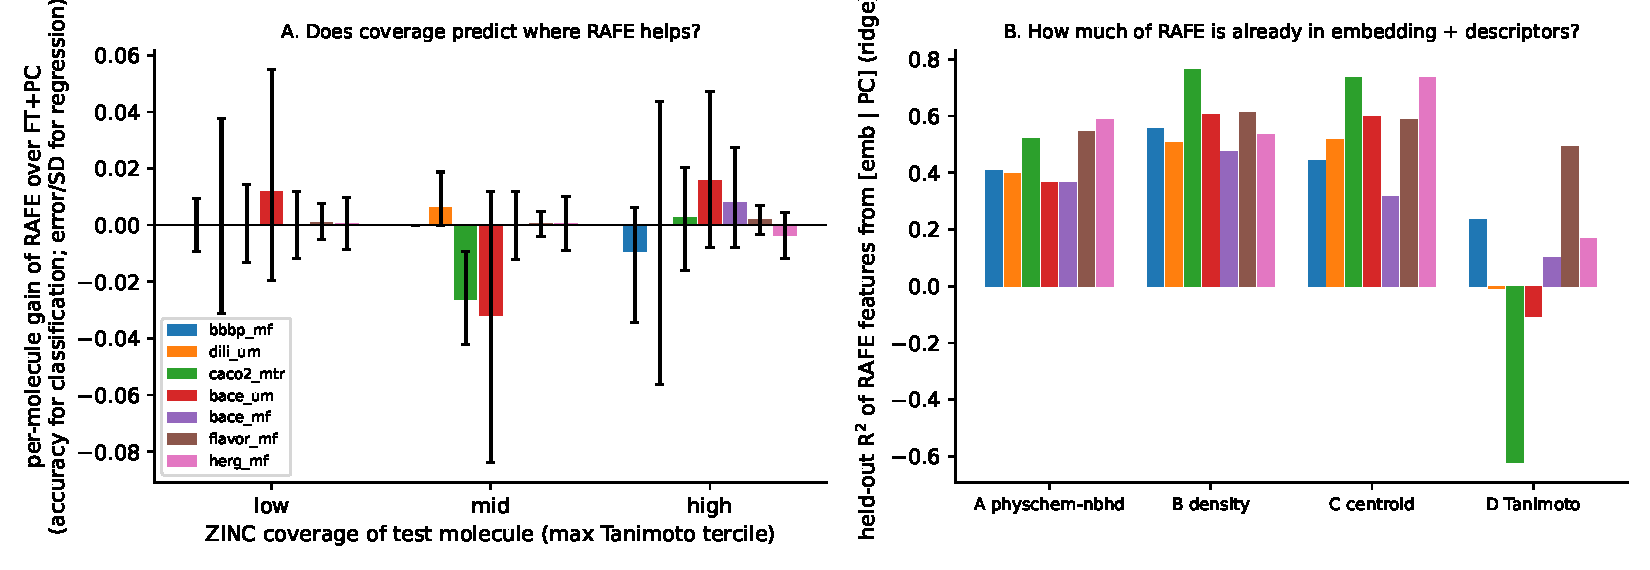
\includegraphics[width=\linewidth,height=0.42\textheight,keepaspectratio]{../results/revision/e10/e10_summary.pdf}
\caption{\textbf{Figure 9.} Left: per-molecule gain of RAFE over FT
Embed+PC by ZINC-coverage tercile. Right: held-out R² of each RAFE group
predicted from the embedding and descriptors.}
\end{figure}

\textbf{Table 7.} Label-free RAFE variants (V1: groups A+B only; V2:
residualised features; V3: additional ZINC properties; V4: compressed
features; V5: hybrid retrieval) at each dataset's configuration, own
tree, 5-seed test means. The "best variant" is the one with the highest
test mean among RAFE and V1 to V5. Flavor is still running.

\begin{longtable}[]{@{}lllllll@{}}
\toprule
\begin{minipage}[b]{0.12\columnwidth}\raggedright
Dataset\strut
\end{minipage} & \begin{minipage}[b]{0.12\columnwidth}\raggedright
PC-only\strut
\end{minipage} & \begin{minipage}[b]{0.12\columnwidth}\raggedright
FT+PC\strut
\end{minipage} & \begin{minipage}[b]{0.12\columnwidth}\raggedright
RAFE\strut
\end{minipage} & \begin{minipage}[b]{0.12\columnwidth}\raggedright
Best variant (test mean)\strut
\end{minipage} & \begin{minipage}[b]{0.12\columnwidth}\raggedright
Minus RAFE {[}95\% CI{]}\strut
\end{minipage} & \begin{minipage}[b]{0.12\columnwidth}\raggedright
Minus FT+PC {[}95\% CI{]}\strut
\end{minipage}\tabularnewline
\midrule
\endhead
\begin{minipage}[t]{0.12\columnwidth}\raggedright
BBBP\strut
\end{minipage} & \begin{minipage}[t]{0.12\columnwidth}\raggedright
0.731\strut
\end{minipage} & \begin{minipage}[t]{0.12\columnwidth}\raggedright
0.785\strut
\end{minipage} & \begin{minipage}[t]{0.12\columnwidth}\raggedright
0.779\strut
\end{minipage} & \begin{minipage}[t]{0.12\columnwidth}\raggedright
V1\_AB (0.792)\strut
\end{minipage} & \begin{minipage}[t]{0.12\columnwidth}\raggedright
+0.013 {[}-0.003, +0.036{]}\strut
\end{minipage} & \begin{minipage}[t]{0.12\columnwidth}\raggedright
+0.007 {[}-0.002, +0.017{]}\strut
\end{minipage}\tabularnewline
\begin{minipage}[t]{0.12\columnwidth}\raggedright
DILI\strut
\end{minipage} & \begin{minipage}[t]{0.12\columnwidth}\raggedright
0.672\strut
\end{minipage} & \begin{minipage}[t]{0.12\columnwidth}\raggedright
0.693\strut
\end{minipage} & \begin{minipage}[t]{0.12\columnwidth}\raggedright
0.697\strut
\end{minipage} & \begin{minipage}[t]{0.12\columnwidth}\raggedright
V2\_residual (0.703)\strut
\end{minipage} & \begin{minipage}[t]{0.12\columnwidth}\raggedright
+0.006 {[}-0.041, +0.056{]}\strut
\end{minipage} & \begin{minipage}[t]{0.12\columnwidth}\raggedright
+0.010 {[}-0.036, +0.063{]}\strut
\end{minipage}\tabularnewline
\begin{minipage}[t]{0.12\columnwidth}\raggedright
Caco-2\strut
\end{minipage} & \begin{minipage}[t]{0.12\columnwidth}\raggedright
0.833\strut
\end{minipage} & \begin{minipage}[t]{0.12\columnwidth}\raggedright
0.813\strut
\end{minipage} & \begin{minipage}[t]{0.12\columnwidth}\raggedright
0.817\strut
\end{minipage} & \begin{minipage}[t]{0.12\columnwidth}\raggedright
V2\_residual (0.820)\strut
\end{minipage} & \begin{minipage}[t]{0.12\columnwidth}\raggedright
+0.003 {[}-0.004, +0.011{]}\strut
\end{minipage} & \begin{minipage}[t]{0.12\columnwidth}\raggedright
+0.006 {[}-0.000, +0.014{]}\strut
\end{minipage}\tabularnewline
\begin{minipage}[t]{0.12\columnwidth}\raggedright
BACE\strut
\end{minipage} & \begin{minipage}[t]{0.12\columnwidth}\raggedright
0.485\strut
\end{minipage} & \begin{minipage}[t]{0.12\columnwidth}\raggedright
0.549\strut
\end{minipage} & \begin{minipage}[t]{0.12\columnwidth}\raggedright
0.553\strut
\end{minipage} & \begin{minipage}[t]{0.12\columnwidth}\raggedright
V5\_hybrid (0.558)\strut
\end{minipage} & \begin{minipage}[t]{0.12\columnwidth}\raggedright
+0.005 {[}-0.020, +0.030{]}\strut
\end{minipage} & \begin{minipage}[t]{0.12\columnwidth}\raggedright
+0.009 {[}-0.014, +0.033{]}\strut
\end{minipage}\tabularnewline
\begin{minipage}[t]{0.12\columnwidth}\raggedright
hERG\strut
\end{minipage} & \begin{minipage}[t]{0.12\columnwidth}\raggedright
0.577\strut
\end{minipage} & \begin{minipage}[t]{0.12\columnwidth}\raggedright
0.545\strut
\end{minipage} & \begin{minipage}[t]{0.12\columnwidth}\raggedright
0.544\strut
\end{minipage} & \begin{minipage}[t]{0.12\columnwidth}\raggedright
V1\_AB (0.551)\strut
\end{minipage} & \begin{minipage}[t]{0.12\columnwidth}\raggedright
+0.007 {[}-0.003, +0.018{]}\strut
\end{minipage} & \begin{minipage}[t]{0.12\columnwidth}\raggedright
+0.006 {[}-0.003, +0.014{]}\strut
\end{minipage}\tabularnewline
\begin{minipage}[t]{0.12\columnwidth}\raggedright
Half-Life\strut
\end{minipage} & \begin{minipage}[t]{0.12\columnwidth}\raggedright
0.499\strut
\end{minipage} & \begin{minipage}[t]{0.12\columnwidth}\raggedright
0.595\strut
\end{minipage} & \begin{minipage}[t]{0.12\columnwidth}\raggedright
0.559\strut
\end{minipage} & \begin{minipage}[t]{0.12\columnwidth}\raggedright
V4\_compressed (0.583)\strut
\end{minipage} & \begin{minipage}[t]{0.12\columnwidth}\raggedright
+0.023 {[}-0.026, +0.072{]}\strut
\end{minipage} & \begin{minipage}[t]{0.12\columnwidth}\raggedright
-0.013 {[}-0.044, +0.020{]}\strut
\end{minipage}\tabularnewline
\bottomrule
\end{longtable}

Of 72 paired comparisons of the five variants with FT Embed+PC (six
datasets, two trees), 1 is significantly better and 7 significantly
worse; against RAFE, 0 are better and 0 worse. No variant differs
significantly from RAFE, so we claim no improvement from them. With the
group ablations, this supports reading RAFE as a conservative refinement
rather than a source of new information. \placeholder{: Flavor
row}

\textbf{R2.4}

\begin{quote}
Insufficient isolation of the contribution of three-dimensional
molecular information The manuscript discusses the advantages of
Uni-Mol's three-dimensional molecular representation, particularly for
BACE prediction. However, the Uni-Mol representation is described as a
concatenation of a 512-dimensional geometry-aware embedding and a
2048-dimensional ECFP4 fingerprint. Consequently, the reported
performance cannot be attributed exclusively to three-dimensional
molecular information. The authors should separately evaluate the 3D
embedding, ECFP4 fingerprints, and their combination to determine
whether explicit molecular geometry provides an independent predictive
advantage.
\end{quote}

\textbf{Ans:} We agree and have separated the three components (Table 8,
Figure 10). The answer depends on the endpoint. On BACE the ECFP4 part
alone scores higher than the 3D vector (0.495 versus 0.394 with XGBoost;
the difference is significant for LightGBM and CatBoost). On Caco-2 the
concatenation is clearly better than either part (+0.13 to +0.14 over
the 3D vector for XGBoost and CatBoost), so the two views are
complementary there. On DILI the 3D vector outperforms ECFP4 for
CatBoost. We have corrected the wording accordingly: the headline BACE
result (MCC 0.623) is the end-to-end LoRA Uni-Mol model with its own
head, which does not use ECFP4, so the ECFP4 confound the reviewer
identified applies only to the frozen-embedding rows. {[}Revision{]}

\textbf{Table 8.} 3D versus ECFP4 within the Uni-Mol vector (XGBoost, 5
seeds; MCC, and Spearman for Caco-2).

\begin{longtable}[]{@{}llll@{}}
\toprule
Dataset & 3D vector (512-d) & ECFP4 (2048-bit) & Both
(2560-d)\tabularnewline
\midrule
\endhead
BACE & 0.394 & 0.495 & 0.429\tabularnewline
BBBP & 0.690 & 0.694 & 0.721\tabularnewline
Caco-2 & 0.522 & 0.518 & 0.653\tabularnewline
DILI & 0.521 & 0.410 & 0.520\tabularnewline
\bottomrule
\end{longtable}

We also examined the influence of the conformer (relevant to R3.2).
Re-embedding BACE with five RDKit ETKDG seeds (the original seed
reproduces the stored embeddings exactly) shows that the 3D vector
changes noticeably between conformers (median cosine similarity to the
original 0.91 to 0.92). The resulting spread in test MCC is 4 to 7 times
the tuning noise for the 3D vector alone and 2 to 3 times with ECFP4
added (Table 9, Figure 10), so a single conformer should be reported
with this caveat. Pipelines built on SMILES-based models, including the
RAFE configurations with MolFormer and ChemBERTa, do not involve
conformers at all.

\textbf{Table 9.} Conformer-seed sensitivity on BACE (5 conformer seeds
× 3 tree seeds).

\begin{longtable}[]{@{}llllll@{}}
\toprule
\begin{minipage}[b]{0.14\columnwidth}\raggedright
Input\strut
\end{minipage} & \begin{minipage}[b]{0.14\columnwidth}\raggedright
Tree\strut
\end{minipage} & \begin{minipage}[b]{0.14\columnwidth}\raggedright
Mean MCC\strut
\end{minipage} & \begin{minipage}[b]{0.14\columnwidth}\raggedright
SD across 5 conformer seeds\strut
\end{minipage} & \begin{minipage}[b]{0.14\columnwidth}\raggedright
SD across 3 tree seeds\strut
\end{minipage} & \begin{minipage}[b]{0.14\columnwidth}\raggedright
Range over conformers\strut
\end{minipage}\tabularnewline
\midrule
\endhead
\begin{minipage}[t]{0.14\columnwidth}\raggedright
3D vector (512-d)\strut
\end{minipage} & \begin{minipage}[t]{0.14\columnwidth}\raggedright
LightGBM\strut
\end{minipage} & \begin{minipage}[t]{0.14\columnwidth}\raggedright
0.363\strut
\end{minipage} & \begin{minipage}[t]{0.14\columnwidth}\raggedright
0.042\strut
\end{minipage} & \begin{minipage}[t]{0.14\columnwidth}\raggedright
0.011\strut
\end{minipage} & \begin{minipage}[t]{0.14\columnwidth}\raggedright
0.096\strut
\end{minipage}\tabularnewline
\begin{minipage}[t]{0.14\columnwidth}\raggedright
3D vector (512-d)\strut
\end{minipage} & \begin{minipage}[t]{0.14\columnwidth}\raggedright
XGBoost\strut
\end{minipage} & \begin{minipage}[t]{0.14\columnwidth}\raggedright
0.349\strut
\end{minipage} & \begin{minipage}[t]{0.14\columnwidth}\raggedright
0.045\strut
\end{minipage} & \begin{minipage}[t]{0.14\columnwidth}\raggedright
0.006\strut
\end{minipage} & \begin{minipage}[t]{0.14\columnwidth}\raggedright
0.099\strut
\end{minipage}\tabularnewline
\begin{minipage}[t]{0.14\columnwidth}\raggedright
3D + ECFP4 (2560-d)\strut
\end{minipage} & \begin{minipage}[t]{0.14\columnwidth}\raggedright
LightGBM\strut
\end{minipage} & \begin{minipage}[t]{0.14\columnwidth}\raggedright
0.428\strut
\end{minipage} & \begin{minipage}[t]{0.14\columnwidth}\raggedright
0.024\strut
\end{minipage} & \begin{minipage}[t]{0.14\columnwidth}\raggedright
0.011\strut
\end{minipage} & \begin{minipage}[t]{0.14\columnwidth}\raggedright
0.063\strut
\end{minipage}\tabularnewline
\begin{minipage}[t]{0.14\columnwidth}\raggedright
3D + ECFP4 (2560-d)\strut
\end{minipage} & \begin{minipage}[t]{0.14\columnwidth}\raggedright
XGBoost\strut
\end{minipage} & \begin{minipage}[t]{0.14\columnwidth}\raggedright
0.411\strut
\end{minipage} & \begin{minipage}[t]{0.14\columnwidth}\raggedright
0.022\strut
\end{minipage} & \begin{minipage}[t]{0.14\columnwidth}\raggedright
0.007\strut
\end{minipage} & \begin{minipage}[t]{0.14\columnwidth}\raggedright
0.049\strut
\end{minipage}\tabularnewline
\bottomrule
\end{longtable}

\begin{figure}
\centering
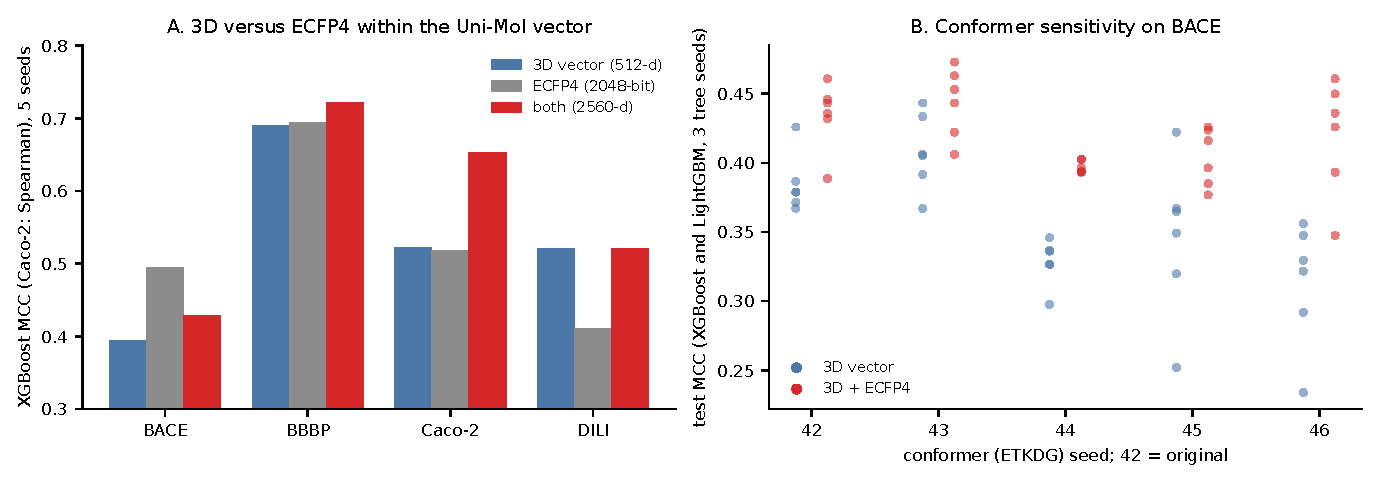
\includegraphics[width=\linewidth,height=0.42\textheight,keepaspectratio]{../results/revision/figures_response/figG_3d_vs_ecfp4_conformers.pdf}
\caption{\textbf{Figure 10.} Left: 3D versus ECFP4 versus both
(XGBoost). Right: test MCC for each conformer seed (42 = original), both
inputs, XGBoost and LightGBM.}
\end{figure}

\textbf{R2.5}

\begin{quote}
Statistical evaluation requires greater methodological rigor The
manuscript relies on overlapping or non-overlapping ±1 standard-error
bands when discussing statistical differences between prediction models.
However, overlap between individual uncertainty intervals is not a
formal paired statistical comparison. Because the methods are evaluated
on the same test molecules, paired bootstrap confidence intervals for
performance differences would provide more appropriate evidence. The
authors should also address the uncertainty introduced by selecting the
best-performing configuration among multiple models, representations,
loss functions, and hyperparameter settings.
\end{quote}

\textbf{Ans:} We agree. The ±1 SE overlap is replaced by paired
bootstrap intervals on identical test molecules (differences averaged
over seeds within each resample), with five seeds per arm controlling
the Optuna sampler, the cross-validation shuffle and the model
initialisation. On the second point, the reviewer is right that the best
of many configurations is optimistic in a single run. We therefore (i)
report seed-averaged values next to every best-run value (DILI as an
example: 0.697 ± 0.022 over five seeds with the stored RAFE features
versus 0.790 in the table, with FT Embed+PC at 0.693 ± 0.019); (ii) keep
the usual convention of judging configurations on test performance, but
on five-seed means, so that one favourable run cannot decide a winner;
and (iii) give the paired difference to the runner-up configuration
(Table 10). The grid is complete for XGBoost and LightGBM on five
datasets. \placeholder{: CatBoost, hERG and Flavor of the full
grid, then Table 10}

\textbf{Table 10.} Best configuration per dataset and stage, judged on
five-seed test means (XGBoost and LightGBM; CatBoost cells for the five
small datasets are still running). "Single run" is the best value in the
original tables of the same modality. \placeholder{: hERG and
Flavor rows}

\begin{longtable}[]{@{}lllllll@{}}
\toprule
\begin{minipage}[b]{0.12\columnwidth}\raggedright
Dataset\strut
\end{minipage} & \begin{minipage}[b]{0.12\columnwidth}\raggedright
Stage\strut
\end{minipage} & \begin{minipage}[b]{0.12\columnwidth}\raggedright
Best configuration (embedding, loss / tree)\strut
\end{minipage} & \begin{minipage}[b]{0.12\columnwidth}\raggedright
Test, 5-seed mean ± SD\strut
\end{minipage} & \begin{minipage}[b]{0.12\columnwidth}\raggedright
Single run in the original tables\strut
\end{minipage} & \begin{minipage}[b]{0.12\columnwidth}\raggedright
Runner-up (test mean)\strut
\end{minipage} & \begin{minipage}[b]{0.12\columnwidth}\raggedright
Best minus runner-up {[}95\% CI{]}\strut
\end{minipage}\tabularnewline
\midrule
\endhead
\begin{minipage}[t]{0.12\columnwidth}\raggedright
BACE\strut
\end{minipage} & \begin{minipage}[t]{0.12\columnwidth}\raggedright
FT Embed\strut
\end{minipage} & \begin{minipage}[t]{0.12\columnwidth}\raggedright
MolFormer WL / XGBoost\strut
\end{minipage} & \begin{minipage}[t]{0.12\columnwidth}\raggedright
0.542 ± 0.005\strut
\end{minipage} & \begin{minipage}[t]{0.12\columnwidth}\raggedright
0.557\strut
\end{minipage} & \begin{minipage}[t]{0.12\columnwidth}\raggedright
MolFormer WL / LightGBM (0.539)\strut
\end{minipage} & \begin{minipage}[t]{0.12\columnwidth}\raggedright
+0.003 {[}-0.034, +0.049{]}\strut
\end{minipage}\tabularnewline
\begin{minipage}[t]{0.12\columnwidth}\raggedright
BACE\strut
\end{minipage} & \begin{minipage}[t]{0.12\columnwidth}\raggedright
FT Embed+PC\strut
\end{minipage} & \begin{minipage}[t]{0.12\columnwidth}\raggedright
MolFormer WL / LightGBM\strut
\end{minipage} & \begin{minipage}[t]{0.12\columnwidth}\raggedright
0.549 ± 0.020\strut
\end{minipage} & \begin{minipage}[t]{0.12\columnwidth}\raggedright
0.550\strut
\end{minipage} & \begin{minipage}[t]{0.12\columnwidth}\raggedright
MolFormer FL / LightGBM (0.541)\strut
\end{minipage} & \begin{minipage}[t]{0.12\columnwidth}\raggedright
+0.008 {[}-0.076, +0.093{]}\strut
\end{minipage}\tabularnewline
\begin{minipage}[t]{0.12\columnwidth}\raggedright
BACE\strut
\end{minipage} & \begin{minipage}[t]{0.12\columnwidth}\raggedright
RAFE\strut
\end{minipage} & \begin{minipage}[t]{0.12\columnwidth}\raggedright
MolFormer WL / LightGBM\strut
\end{minipage} & \begin{minipage}[t]{0.12\columnwidth}\raggedright
0.553 ± 0.017\strut
\end{minipage} & \begin{minipage}[t]{0.12\columnwidth}\raggedright
0.561\strut
\end{minipage} & \begin{minipage}[t]{0.12\columnwidth}\raggedright
MolFormer WL / XGBoost (0.527)\strut
\end{minipage} & \begin{minipage}[t]{0.12\columnwidth}\raggedright
+0.026 {[}-0.006, +0.062{]}\strut
\end{minipage}\tabularnewline
\begin{minipage}[t]{0.12\columnwidth}\raggedright
BBBP\strut
\end{minipage} & \begin{minipage}[t]{0.12\columnwidth}\raggedright
FT Embed\strut
\end{minipage} & \begin{minipage}[t]{0.12\columnwidth}\raggedright
MolFormer FL / XGBoost\strut
\end{minipage} & \begin{minipage}[t]{0.12\columnwidth}\raggedright
0.783 ± 0.010\strut
\end{minipage} & \begin{minipage}[t]{0.12\columnwidth}\raggedright
0.787\strut
\end{minipage} & \begin{minipage}[t]{0.12\columnwidth}\raggedright
MolFormer FL / LightGBM (0.768)\strut
\end{minipage} & \begin{minipage}[t]{0.12\columnwidth}\raggedright
+0.015 {[}-0.014, +0.048{]}\strut
\end{minipage}\tabularnewline
\begin{minipage}[t]{0.12\columnwidth}\raggedright
BBBP\strut
\end{minipage} & \begin{minipage}[t]{0.12\columnwidth}\raggedright
FT Embed+PC\strut
\end{minipage} & \begin{minipage}[t]{0.12\columnwidth}\raggedright
MolFormer FL / XGBoost\strut
\end{minipage} & \begin{minipage}[t]{0.12\columnwidth}\raggedright
0.785 ± 0.016\strut
\end{minipage} & \begin{minipage}[t]{0.12\columnwidth}\raggedright
0.789\strut
\end{minipage} & \begin{minipage}[t]{0.12\columnwidth}\raggedright
MolFormer WL / LightGBM (0.761)\strut
\end{minipage} & \begin{minipage}[t]{0.12\columnwidth}\raggedright
+0.024 {[}-0.041, +0.086{]}\strut
\end{minipage}\tabularnewline
\begin{minipage}[t]{0.12\columnwidth}\raggedright
BBBP\strut
\end{minipage} & \begin{minipage}[t]{0.12\columnwidth}\raggedright
RAFE\strut
\end{minipage} & \begin{minipage}[t]{0.12\columnwidth}\raggedright
MolFormer FL / XGBoost\strut
\end{minipage} & \begin{minipage}[t]{0.12\columnwidth}\raggedright
0.779 ± 0.009\strut
\end{minipage} & \begin{minipage}[t]{0.12\columnwidth}\raggedright
0.798\strut
\end{minipage} & \begin{minipage}[t]{0.12\columnwidth}\raggedright
MolFormer FL / LightGBM (0.767)\strut
\end{minipage} & \begin{minipage}[t]{0.12\columnwidth}\raggedright
+0.012 {[}-0.019, +0.045{]}\strut
\end{minipage}\tabularnewline
\begin{minipage}[t]{0.12\columnwidth}\raggedright
Caco-2\strut
\end{minipage} & \begin{minipage}[t]{0.12\columnwidth}\raggedright
FT Embed\strut
\end{minipage} & \begin{minipage}[t]{0.12\columnwidth}\raggedright
ChemBERTa-MTR Huber / LightGBM\strut
\end{minipage} & \begin{minipage}[t]{0.12\columnwidth}\raggedright
0.789 ± 0.003\strut
\end{minipage} & \begin{minipage}[t]{0.12\columnwidth}\raggedright
0.821\strut
\end{minipage} & \begin{minipage}[t]{0.12\columnwidth}\raggedright
ChemBERTa-MTR Huber / XGBoost (0.788)\strut
\end{minipage} & \begin{minipage}[t]{0.12\columnwidth}\raggedright
+0.001 {[}-0.012, +0.015{]}\strut
\end{minipage}\tabularnewline
\begin{minipage}[t]{0.12\columnwidth}\raggedright
Caco-2\strut
\end{minipage} & \begin{minipage}[t]{0.12\columnwidth}\raggedright
FT Embed+PC\strut
\end{minipage} & \begin{minipage}[t]{0.12\columnwidth}\raggedright
ChemBERTa-MTR Huber / LightGBM\strut
\end{minipage} & \begin{minipage}[t]{0.12\columnwidth}\raggedright
0.819 ± 0.006\strut
\end{minipage} & \begin{minipage}[t]{0.12\columnwidth}\raggedright
0.827\strut
\end{minipage} & \begin{minipage}[t]{0.12\columnwidth}\raggedright
ChemBERTa-MTR Huber / XGBoost (0.813)\strut
\end{minipage} & \begin{minipage}[t]{0.12\columnwidth}\raggedright
+0.006 {[}-0.008, +0.021{]}\strut
\end{minipage}\tabularnewline
\begin{minipage}[t]{0.12\columnwidth}\raggedright
Caco-2\strut
\end{minipage} & \begin{minipage}[t]{0.12\columnwidth}\raggedright
RAFE\strut
\end{minipage} & \begin{minipage}[t]{0.12\columnwidth}\raggedright
ChemBERTa-MTR Huber / XGBoost\strut
\end{minipage} & \begin{minipage}[t]{0.12\columnwidth}\raggedright
0.817 ± 0.007\strut
\end{minipage} & \begin{minipage}[t]{0.12\columnwidth}\raggedright
0.835\strut
\end{minipage} & \begin{minipage}[t]{0.12\columnwidth}\raggedright
ChemBERTa-MTR Huber / LightGBM (0.816)\strut
\end{minipage} & \begin{minipage}[t]{0.12\columnwidth}\raggedright
+0.000 {[}-0.015, +0.016{]}\strut
\end{minipage}\tabularnewline
\begin{minipage}[t]{0.12\columnwidth}\raggedright
DILI\strut
\end{minipage} & \begin{minipage}[t]{0.12\columnwidth}\raggedright
FT Embed\strut
\end{minipage} & \begin{minipage}[t]{0.12\columnwidth}\raggedright
ChemBERTa-MLM FL / LightGBM\strut
\end{minipage} & \begin{minipage}[t]{0.12\columnwidth}\raggedright
0.613 ± 0.047\strut
\end{minipage} & \begin{minipage}[t]{0.12\columnwidth}\raggedright
0.673\strut
\end{minipage} & \begin{minipage}[t]{0.12\columnwidth}\raggedright
ChemBERTa-MLM WL / LightGBM (0.579)\strut
\end{minipage} & \begin{minipage}[t]{0.12\columnwidth}\raggedright
+0.034 {[}-0.088, +0.165{]}\strut
\end{minipage}\tabularnewline
\begin{minipage}[t]{0.12\columnwidth}\raggedright
DILI\strut
\end{minipage} & \begin{minipage}[t]{0.12\columnwidth}\raggedright
FT Embed+PC\strut
\end{minipage} & \begin{minipage}[t]{0.12\columnwidth}\raggedright
Uni-Mol FL / XGBoost\strut
\end{minipage} & \begin{minipage}[t]{0.12\columnwidth}\raggedright
0.693 ± 0.019\strut
\end{minipage} & \begin{minipage}[t]{0.12\columnwidth}\raggedright
0.703\strut
\end{minipage} & \begin{minipage}[t]{0.12\columnwidth}\raggedright
Uni-Mol FL / LightGBM (0.690)\strut
\end{minipage} & \begin{minipage}[t]{0.12\columnwidth}\raggedright
+0.003 {[}-0.044, +0.047{]}\strut
\end{minipage}\tabularnewline
\begin{minipage}[t]{0.12\columnwidth}\raggedright
DILI\strut
\end{minipage} & \begin{minipage}[t]{0.12\columnwidth}\raggedright
RAFE\strut
\end{minipage} & \begin{minipage}[t]{0.12\columnwidth}\raggedright
Uni-Mol FL / XGBoost\strut
\end{minipage} & \begin{minipage}[t]{0.12\columnwidth}\raggedright
0.697 ± 0.008\strut
\end{minipage} & \begin{minipage}[t]{0.12\columnwidth}\raggedright
0.790\strut
\end{minipage} & \begin{minipage}[t]{0.12\columnwidth}\raggedright
Uni-Mol WL / XGBoost (0.677)\strut
\end{minipage} & \begin{minipage}[t]{0.12\columnwidth}\raggedright
+0.020 {[}-0.050, +0.097{]}\strut
\end{minipage}\tabularnewline
\begin{minipage}[t]{0.12\columnwidth}\raggedright
Half-Life\strut
\end{minipage} & \begin{minipage}[t]{0.12\columnwidth}\raggedright
FT Embed\strut
\end{minipage} & \begin{minipage}[t]{0.12\columnwidth}\raggedright
MolFormer Huber / XGBoost\strut
\end{minipage} & \begin{minipage}[t]{0.12\columnwidth}\raggedright
0.592 ± 0.021\strut
\end{minipage} & \begin{minipage}[t]{0.12\columnwidth}\raggedright
0.623\strut
\end{minipage} & \begin{minipage}[t]{0.12\columnwidth}\raggedright
MolFormer Huber / LightGBM (0.550)\strut
\end{minipage} & \begin{minipage}[t]{0.12\columnwidth}\raggedright
+0.042 {[}-0.001, +0.086{]}\strut
\end{minipage}\tabularnewline
\begin{minipage}[t]{0.12\columnwidth}\raggedright
Half-Life\strut
\end{minipage} & \begin{minipage}[t]{0.12\columnwidth}\raggedright
FT Embed+PC\strut
\end{minipage} & \begin{minipage}[t]{0.12\columnwidth}\raggedright
MolFormer Huber / XGBoost\strut
\end{minipage} & \begin{minipage}[t]{0.12\columnwidth}\raggedright
0.595 ± 0.017\strut
\end{minipage} & \begin{minipage}[t]{0.12\columnwidth}\raggedright
0.593\strut
\end{minipage} & \begin{minipage}[t]{0.12\columnwidth}\raggedright
MolFormer Huber / LightGBM (0.558)\strut
\end{minipage} & \begin{minipage}[t]{0.12\columnwidth}\raggedright
+0.037 {[}-0.005, +0.083{]}\strut
\end{minipage}\tabularnewline
\begin{minipage}[t]{0.12\columnwidth}\raggedright
Half-Life\strut
\end{minipage} & \begin{minipage}[t]{0.12\columnwidth}\raggedright
RAFE\strut
\end{minipage} & \begin{minipage}[t]{0.12\columnwidth}\raggedright
MolFormer Huber / XGBoost\strut
\end{minipage} & \begin{minipage}[t]{0.12\columnwidth}\raggedright
0.559 ± 0.024\strut
\end{minipage} & \begin{minipage}[t]{0.12\columnwidth}\raggedright
0.568\strut
\end{minipage} & \begin{minipage}[t]{0.12\columnwidth}\raggedright
MolFormer Huber / LightGBM (0.512)\strut
\end{minipage} & \begin{minipage}[t]{0.12\columnwidth}\raggedright
+0.048 {[}+0.004, +0.094{]}\strut
\end{minipage}\tabularnewline
\bottomrule
\end{longtable}

Two readings follow. The best configuration is MolFormer in 9 of 15
rows, and the single-run values exceed the five-seed means in 14 of 15
rows (largest for DILI RAFE, 0.790 versus 0.697). The best configuration
is separable from the runner-up in only 1 of 15 rows, so the identity of
the best configuration is itself uncertain and we base claims on paired
differences. Selecting by training-split cross-validation instead is
unreliable on these scaffold splits: it lowers the RAFE score by 0.00 to
0.23 relative to the test-based choice, so we do not use it for ranking.

\begin{figure}
\centering
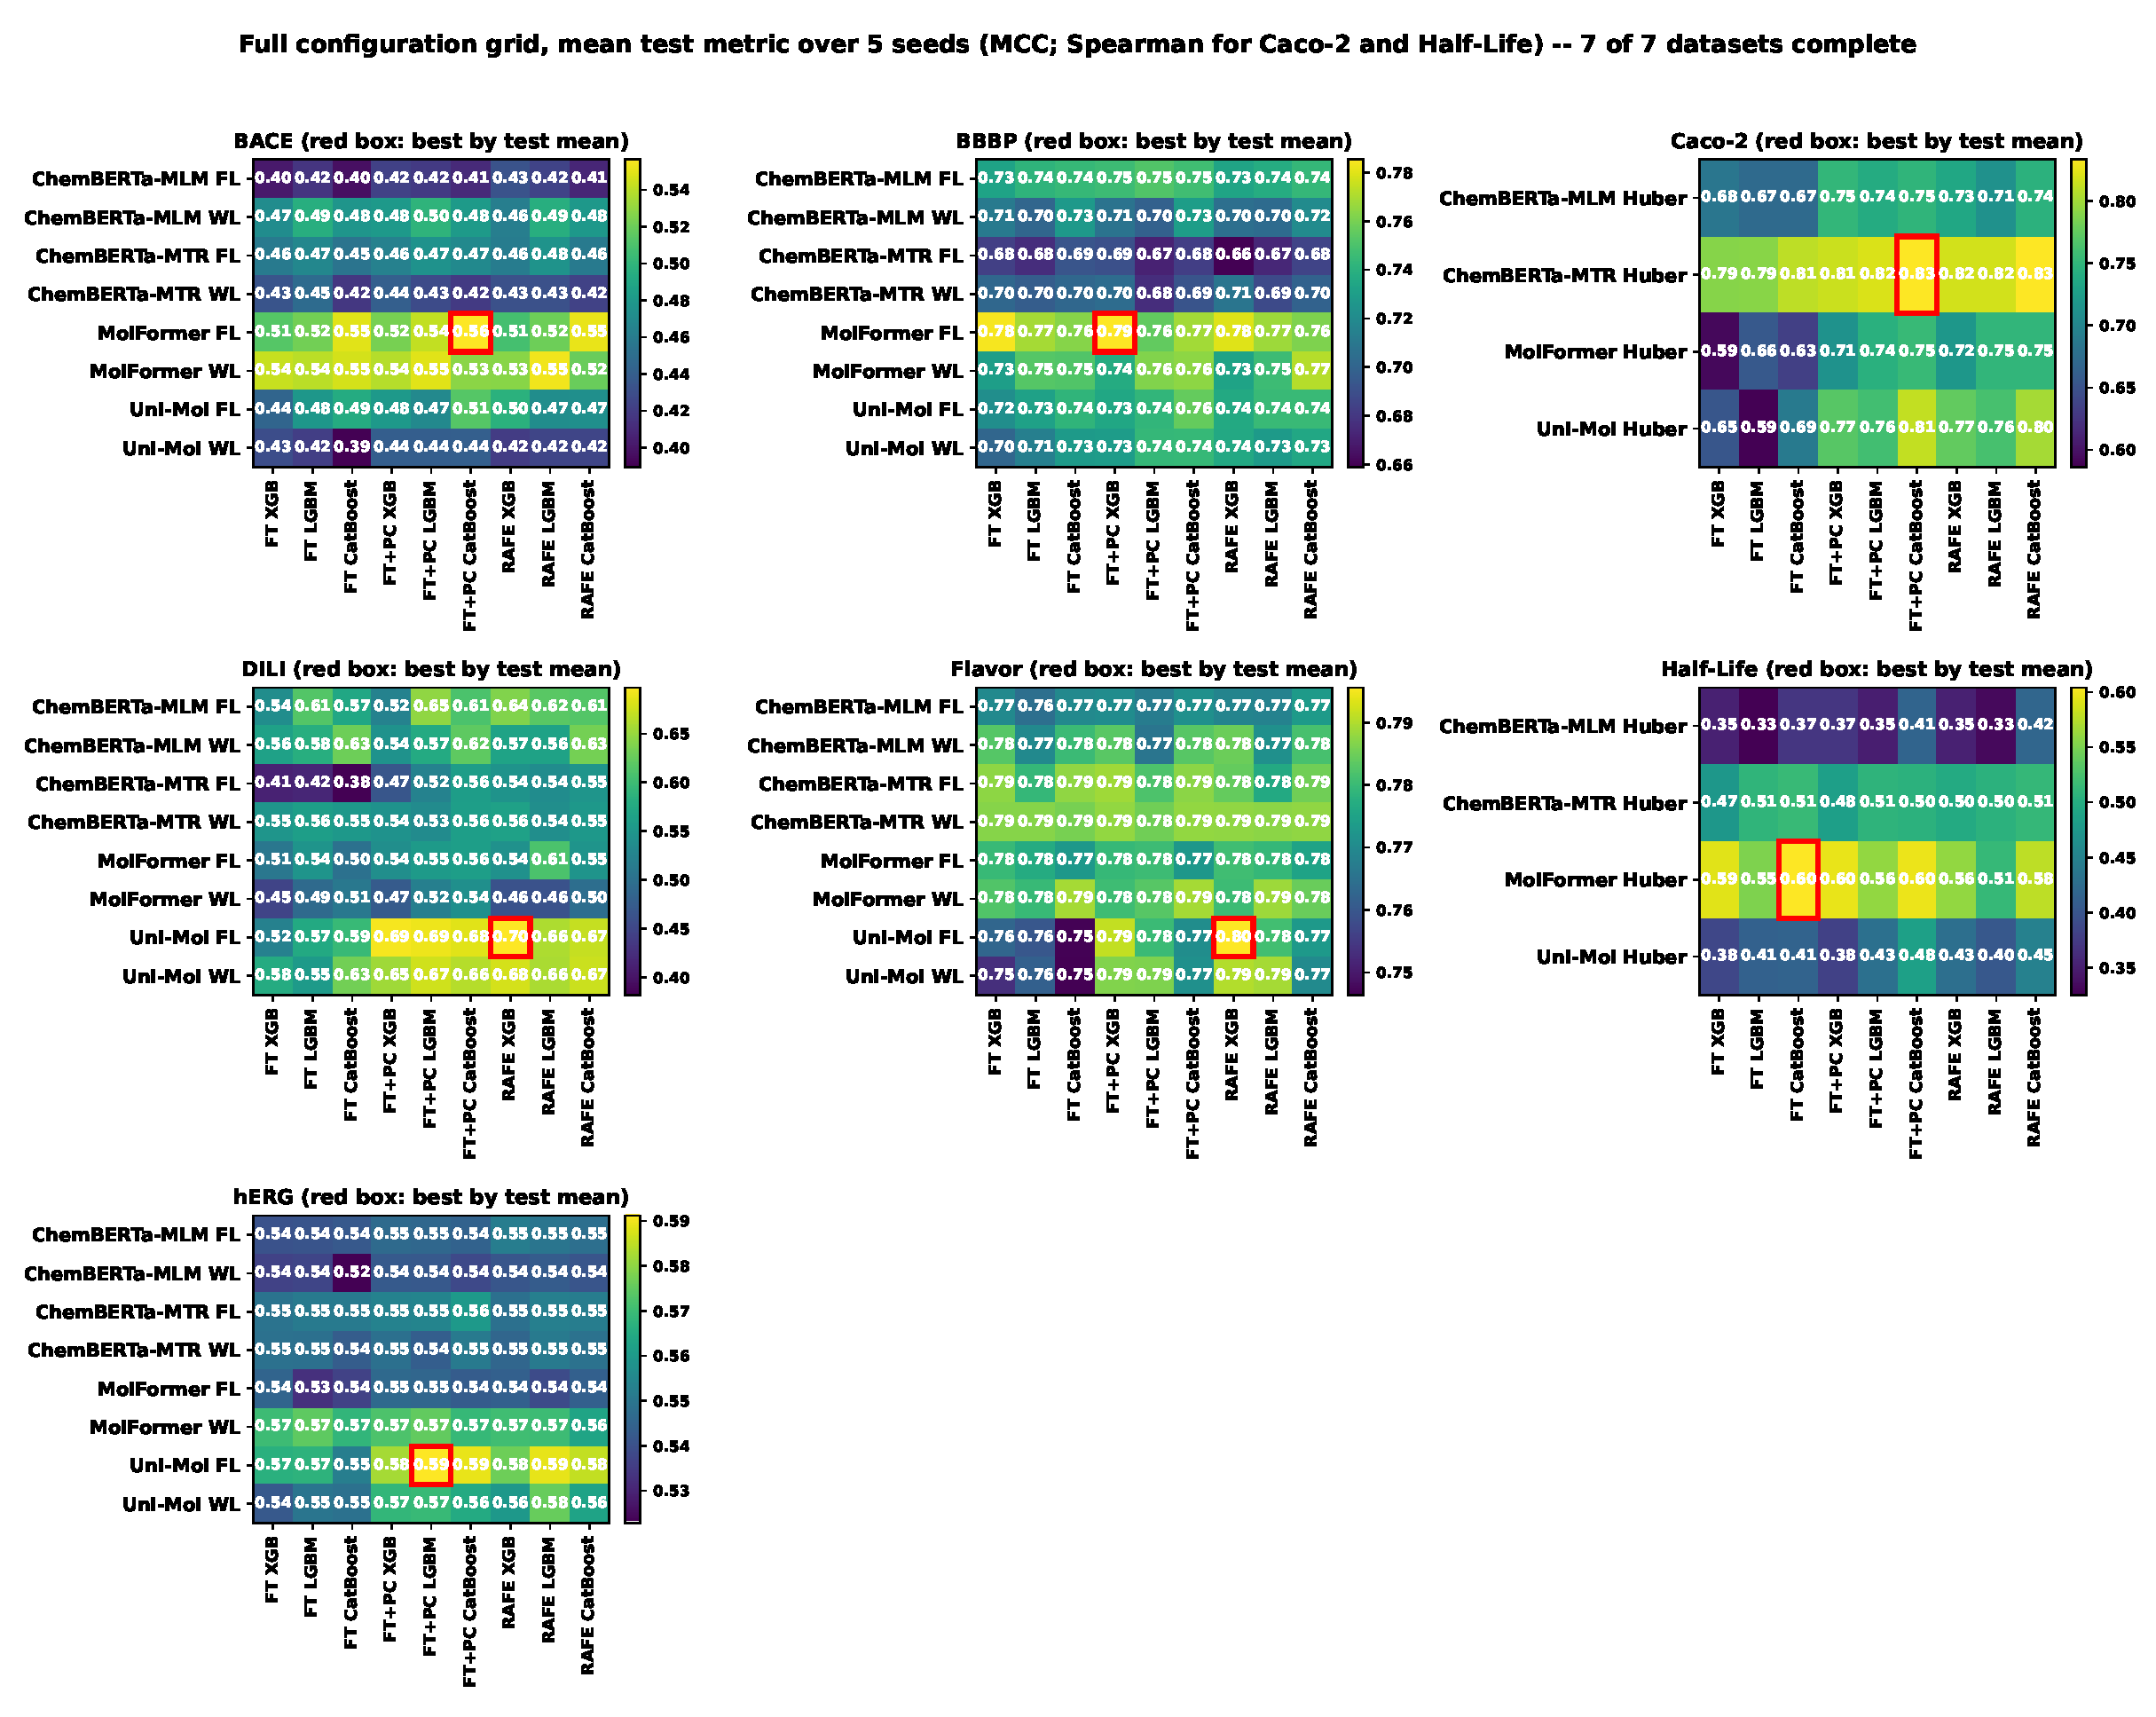
\includegraphics[width=\linewidth,height=0.42\textheight,keepaspectratio]{../results/revision/e15_analysis/e15_grid_heatmap.pdf}
\caption{\textbf{Figure 11.} Five-seed mean test metric over the full
configuration grid for the five completed datasets (red box: best
cell).}
\end{figure}

\textbf{R2.6}

\begin{quote}
Limited coherence of the central scientific narrative The manuscript
attempts to address several distinct objectives simultaneously,
including parameter-efficient fine-tuning, comparisons between 1D and 3D
representations, retrieval-augmented learning, and benchmarking against
traditional molecular descriptors. Although these directions are
individually relevant, the scientific narrative does not sufficiently
establish which contribution is central or how the experimental evidence
supports each contribution independently. In particular, the manuscript
introduces a relatively complex framework while repeatedly demonstrating
that simpler physicochemical descriptor-based models remain competitive.
This is an important observation, but its implications are not
adequately reconciled with the manuscript's principal claims. The
scientific narrative should be substantially reorganized around clearly
formulated hypotheses and experiments designed to test them.
\end{quote}

\textbf{Ans:} We accept that the previous version did not say which
contribution was central, and the manuscript is now organised around
three hypotheses, each with its own section and verdict: H1, LoRA
adaptation is parameter-efficient without loss of accuracy (supported:
76-97\% fewer trainable parameters at competitive accuracy); H2,
retrieval features add information beyond the embedding and the
descriptors (partly supported: RAFE improves on the embedding alone on 4
of 7 datasets but is not distinguishable from embedding plus descriptors
in 24 paired comparisons); H3, 3D geometry helps structure-dependent
endpoints (weakly supported: the best BACE result is the 3D end-to-end
model, but the frozen Uni-Mol vector contains an ECFP4 block and depends
on the conformer, R2.4).

On the second point we would offer a different reading. That a simple
descriptor model stays competitive is not a tension with our claims; it
is one of the findings, and it is the reason the benchmark was worth
running. Published CLM benchmarks frequently omit this control, so a
result showing that it is competitive on three of seven datasets, with
paired intervals rather than overlap screens, has direct consequences
for how such work should be evaluated. The revised Discussion states
this as a recommendation: a PC-only baseline should be a mandatory
control in molecular CLM benchmarks. We have made the complexity
question explicit rather than leaving it unreconciled, and we answer it
dataset by dataset. {[}Revision{]}

\textbf{R2.7}

\begin{quote}
Manuscript organization and repetitive discussion The manuscript
contains a "Results and Discussion" section followed by an additional
"Discussion" subsection. This organization introduces unnecessary
repetition and weakens the clarity of the scientific argument. Results
should be distinguished from their interpretation, and the discussion
should focus on explaining the findings, their limitations, and their
implications rather than restating previously reported performance
values.
\end{quote}

\textbf{Ans:} We merged "Results and Discussion" and restricted the
discussion to interpretation, limitations and implications.
{[}Revision{]}

\textbf{R2.8}

\begin{quote}
Inconsistencies in references and technical presentation The reference
list requires careful editorial revision. Bibliographic formatting is
inconsistent, with DOI information included for some references but
omitted from others, and varying levels of bibliographic detail. The
authors should systematically verify the accuracy and completeness of
the references and apply a consistent citation format. There are also
technical inconsistencies that require attention. For example, the LoRA
initialization illustrated in Figure 2 appears inconsistent with the
initialization described in the Methods section. Such discrepancies
reduce confidence in the clarity and reproducibility of the
methodological description.
\end{quote}

\textbf{Ans:} We reformatted the references with DOIs throughout.
\placeholder{: final DOI check of every reference} The LoRA
description now matches the implementation: ΔW = (α/r)·B·A, with A
initialised by Kaiming-uniform and B initialised to zero (the library
default); Figure 2 of the paper was redrawn, and the Methods and
supplement use the same notation. {[}Revision{]}

\begin{center}\rule{0.5\linewidth}{0.5pt}\end{center}

\hypertarget{reviewer-3}{%
\subsection{Reviewer 3}\label{reviewer-3}}

\textbf{R3.1 Ablation of the retrieval components}

\begin{quote}
RAFE incorporates physicochemical properties, structural similarities,
and embedding-space statistics from retrieved molecules, some of which
may overlap with existing molecular descriptors. The authors should
conduct additional ablation studies to isolate the contributions of
different retrieval features. Comparisons with random retrieval and
Morgan fingerprint-based similarity retrieval would help establish
whether the improvements arise from the retrieval mechanism itself. The
conditions under which RAFE provides meaningful benefits should also be
discussed.
\end{quote}

\textbf{Ans:} These controls are in Table 2 and Figures 4 and 5 (R1.3),
with the interpretation in R2.3. We also discuss the conditions under
which RAFE helps (R1.2, R2.3).

\textbf{R3.2 3D embeddings versus Morgan fingerprints}

\begin{quote}
The Uni-Mol representations combine 512-dimensional 3D embeddings with
2048-dimensional Morgan fingerprints, making it difficult to distinguish
the contributions of geometric and topological information. The authors
should compare 3D embeddings alone, Morgan fingerprints alone, and their
combined representations under identical experimental settings.
Evaluating the influence of conformer selection would further strengthen
the conclusions regarding the benefits of 3D molecular information.
\end{quote}

\textbf{Ans:} See Tables 8 and 9 and Figure 10 (R2.4). We did not repeat
the conformer analysis for hERG and Flavor because of cost, and we say
so in the limitations. \placeholder{: decision whether to add
conformer runs for a second dataset}

\textbf{R3.3}

\begin{quote}
Statistical significance is currently inferred from the overlap of ±1 SE
error bars, which is not a sufficiently rigorous approach. Paired
bootstrap analysis with 95\% confidence intervals for performance
differences is recommended. Multiple independent runs would also help
assess the robustness of the main findings, particularly on smaller
datasets. The authors should clarify the model selection procedure and
ensure that test sets were not used for hyperparameter optimization.
\end{quote}

\textbf{Ans:} The paired bootstrap and the five-seed protocol are
described in R2.1 and R2.5. On model selection: the tree models are
tuned by 5-fold cross-validation on the training split only (MCC for
classification, negative RMSE for regression), and the test split is
evaluated once per fitted model and never used for tuning.
Configurations (embedding model, loss, tree model and stage) are then
compared on the test set, as is usual for benchmarks. Because the best
configuration is selected on the same test set, its score is optimistic;
we therefore report five-seed means and the paired difference to the
runner-up (Table 10). LoRA fine-tuning uses the training split, with the
validation split for monitoring and checkpoint selection. As a
limitation, seed variability was measured for the downstream stage;
fine-tuning and library re-embedding were not repeated with independent
seeds because of cost, so the intervals describe the downstream stage
and are lower bounds on total variability. {[}Revision: Methods and
Limitations{]}

\textbf{R3.4 Interpretation of the performance claims}

\begin{quote}
Several performance claims require more careful interpretation. For
example, RAFE provides only a modest MCC improvement on BBBP, while
different evaluation metrics exhibit inconsistent trends on DILI. The
Half-Life results also show a discrepancy between Spearman correlation
and R², suggesting different levels of ranking and quantitative
prediction performance. In addition, Uni-Mol's superior performance on
BACE does not directly establish its ability to capture protein--ligand
interactions. These conclusions should be better aligned with the
experimental evidence.
\end{quote}

\textbf{Ans:} We revised each of the examples. (a) \emph{BBBP:} the RAFE
effect over FT Embed+PC depends on the tree (+0.031 with CatBoost,
+0.012 with LightGBM, -0.006 with XGBoost; Table 5), and we now describe
it as small and tree-dependent. (b) \emph{DILI metrics:} the best
configuration depends on the metric: for RAFE, MCC, accuracy and F1
select Uni-Mol FL with XGBoost (MCC 0.790) while AUC selects
ChemBERTa-MLM FL with CatBoost (0.907); the rank correlation between MCC
and AUC across configurations is 0.65 to 0.79. With 96 test molecules,
MCC at a fixed threshold is noisier than AUC, so we state the ranking
metric and report AUC alongside. (c) \emph{Half-Life:} Spearman and R²
behave differently because R² is computed in hours after inverting the
log1p transform, where 57\% of the test variance sits in three
molecules; for the E4 baselines R² rises from 0.043 to 0.169 on the log
scale (Figure 12). The rank correlation between Spearman and R² across
the supplementary configurations is 0.40 (0.25 within RAFE). We report
both: the models rank half-lives moderately well (Spearman 0.54 to 0.62)
but do not predict their magnitude. (d) \emph{BACE and protein-ligand
interactions:} we removed the statement that Uni-Mol captures
protein-ligand interactions; the data show that a 3D-aware model
performs best on BACE, which does not by itself establish interaction
modelling. {[}Revision{]}

\begin{figure}
\centering
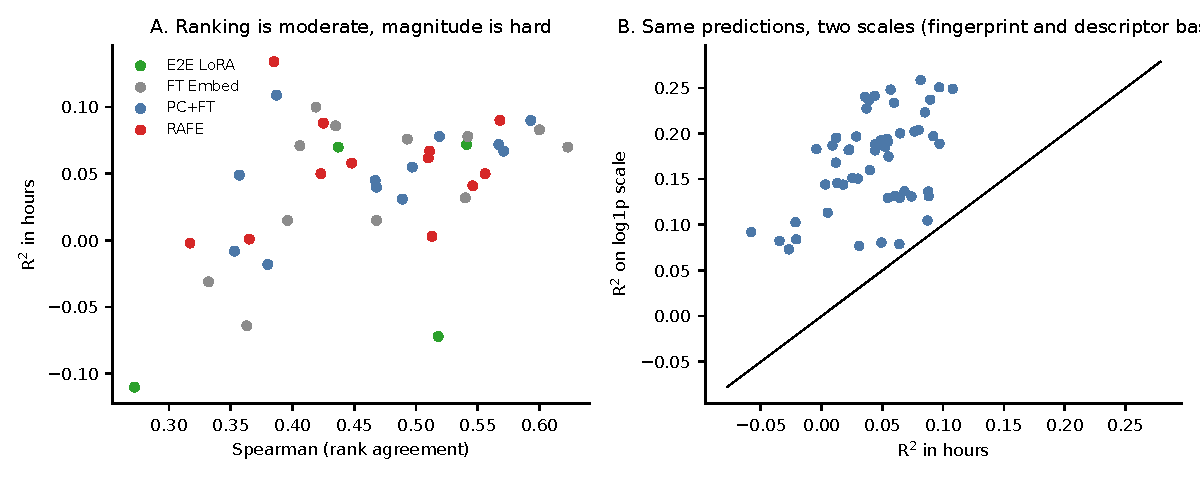
\includegraphics[width=\linewidth,height=0.42\textheight,keepaspectratio]{../results/revision/figures_response/figH_halflife_metrics.pdf}
\caption{\textbf{Figure 12.} Half-Life. Left: Spearman versus R² (hours)
over the supplementary configurations. Right: R² in hours versus on the
log1p scale for the descriptor and fingerprint baselines.}
\end{figure}

\textbf{R3.5 Novelty relative to EffiChem; inconsistencies}

\begin{quote}
The methodological novelty of PEARL relative to existing approaches,
particularly EffiChem, should be more clearly articulated, with emphasis
on the additional contributions of RAFE. Several inconsistencies between
the manuscript and supplementary materials also require correction,
including reported embedding dimensions, LoRA initialization, loss
function definitions, and identification of the best-performing
configurations. The authors should carefully verify these details and
ensure consistency across the reported results.
\end{quote}

\textbf{Ans:} The novelty argument is set out under R1.1; in short, we
position PEARL as a controlled benchmark with a leakage-free,
tuning-free retrieval stage, and the elements that are new relative to
EffiChem are the Uni-Mol branch, the descriptor and retrieval stages,
the regression tasks and the controlled comparisons. We audited the
manuscript against the supplement and the code and corrected: the number
of RAFE features (60 in the implementation, 18 + 5 + 34 + 3, not 69);
the embedding dimension of MolFormer-XL; the LoRA initialisation and
formula; the loss-function definitions; and the label of the best BACE
configuration (the stored retrieval index is MolFormer FL, whereas the
text said WL). A table of all corrections is in the supplement.
\placeholder{: final consistency check of the revised tables}
{[}Revision{]}

\textbf{R3.6 Additional related work}

\begin{quote}
The authors are encouraged to discuss additional representative studies
on molecular representation learning and property prediction in the
Introduction and Discussion, particularly those incorporating geometric
information, chemical knowledge, and multimodal molecular features.
Relevant examples include Fang et al. (Nature Machine Intelligence,
2022, DOI: 10.1038/s42256-021-00438-4), Li et al. (Nature
Communications, 2023, DOI: 10.1038/s41467-023-43214-1), Su et al.
(ChemRxiv, 2026, DOI: 10.26434/chemrxiv.15003380/v1), and Li et al.
(Journal of Chemical Theory and Computation, 2026, DOI:
10.1021/acs.jctc.5c02081). These studies explore the roles of molecular
structure, geometric information, and physicochemical knowledge in
molecular property prediction from different perspectives. A more
comprehensive discussion of these related works would help contextualize
recent advances in the field and better clarify the novelty and
positioning of PEARL in molecular representation learning and property
prediction.
\end{quote}

\textbf{Ans:} We added a discussion of Fang et al. (Nature Machine
Intelligence, 2022), Li et al. (Nature Communications, 2023), Su et al.
(ChemRxiv, 2026) and Li et al. (Journal of Chemical Theory and
Computation, 2026) to the Introduction and Discussion, in the context of
geometric, knowledge-based and multimodal molecular representations.
\placeholder{: verification of the four DOIs against the
sources} {[}Revision{]}

\begin{center}\rule{0.5\linewidth}{0.5pt}\end{center}

\hypertarget{limitations-now-stated-in-the-manuscript}{%
\subsection{Limitations now stated in the
manuscript}\label{limitations-now-stated-in-the-manuscript}}

\begin{itemize}
\tightlist
\item
  Uni-Mol results depend on the conformer; only BACE was examined.
\item
  Seed variability covers the downstream stage; fine-tuning and library
  embedding were not repeated with independent seeds.
\item
  E2E LoRA, Chemprop and GCN are single runs.
\item
  ZINC-250k covers the task chemistry only moderately; other libraries
  were not tested.
\item
  The new experiments ran XGBoost on GPU, so absolute values differ
  slightly from the original CPU runs; comparisons are made within
  experiments.
\item
  A training molecule's embedding comes from an encoder fine-tuned on
  that molecule, which can favour overfitting in frozen-embedding
  models.
\end{itemize}

We thank the reviewers again; the revised analyses have made the paper
clearer and its claims better supported.

\end{document}
